%% Dokumentenklasse (Koma Script) -----------------------------------------
\documentclass[%
   %draft,     % Entwurfsstadium
   final,      % fertiges Dokument
   12pt,
   headings=big,       % gro�e �berschriften
   ngerman,           % wird an andere Pakete weitergereicht
   a4paper,
   BCOR5mm,          % Zusaetzlicher Rand auf der Innenseite
   DIV12,            % Seitengroesse (siehe Koma Skript Dokumentation !)
   %DIV=calc,
   1.1headlines,     % Zeilenanzahl der Kopfzeilen
   pagesize,         % Schreibt die Papiergroesse in die Datei.
   oneside,
%   twoside,          % Seitenraender f�r zweiseitiges Layout
   openright,        % Kapitel beginnen immer auf der rechten Seite
   titlepage,        % Titel als einzelne Seite ('titlepage' Umgebung) 
   parskip=false,        % Einger�ckt (Standard)
   headsepline,      % Linie unter Kolumnentitel
   chapterprefix=false,  % keine Ausgabe von 'Kapitel:'      
	 toc=bibliography, % Literaturverzeichnis ins Inhaltsverzeichnis
	 toc=graduated,		% eingereuckte Gliederung des Inhaltsverzeichnisses
	 toc=listof,			% Tabellen- und Abbildungsverzeichnis ins Inhaltsverzeichnis
   numbers=noenddot, % �erschriftnummerierung ohne Punkt, siehe DUDEN !
   %cleardoubleplain=plain,
	 footinclude=false,
   %fleqn,            % Formeln werden linksbuendig angezeigt
]{scrbook}%     Klassen: scrartcl, scrreprt, scrbook
% -------------------------------------------------------------------------


\usepackage[latin1]{inputenc}



%%% Preambel
%%% Frei nach einer Vorlage von Matthias Pospiech
%%% Modifiziert von Frederik Beer



%%% Packages for LaTeX -programming
% Define commands that don't eat spaces.
\usepackage{xspace}
% IfThenElse
\usepackage{ifthen}
%%% Doc: ftp://tug.ctan.org/pub/tex-archive/macros/latex/contrib/oberdiek/ifpdf.sty
% command for testing for pdf-creation
\usepackage{ifpdf} %\ifpdf \else \fi

%%% Internal Commands: ----------------------------------------------
\makeatletter
%
\providecommand{\IfPackageLoaded}[2]{\@ifpackageloaded{#1}{#2}{}}
\providecommand{\IfPackageNotLoaded}[2]{\@ifpackageloaded{#1}{}{#2}}
\providecommand{\IfElsePackageLoaded}[3]{\@ifpackageloaded{#1}{#2}{#3}}
%
\newboolean{chapteravailable}%
\setboolean{chapteravailable}{false}%

\ifcsname chapter\endcsname
  \setboolean{chapteravailable}{true}%
\else
  \setboolean{chapteravailable}{false}%
\fi


\providecommand{\IfChapterDefined}[1]{\ifthenelse{\boolean{chapteravailable}}{#1}{}}%
\providecommand{\IfElseChapterDefined}[2]{\ifthenelse{\boolean{chapteravailable}}{#1}{#2}}%

\providecommand{\IfDefined}[2]{%
\ifcsname #1\endcsname
   #2 %
\else
     % do nothing
\fi
}
%
% Check for 'draft' mode - commands.
\newcommand{\IfNotDraft}[1]{\ifx\@draft\@undefined #1 \fi}
\newcommand{\IfNotDraftElse}[2]{\ifx\@draft\@undefined #1 \else #2 \fi}
\newcommand{\IfDraft}[1]{\ifx\@draft\@undefined \else #1 \fi}
%



% Definde frontmatter, mainmatter and backmatter if not defined
\@ifundefined{frontmatter}{%
   \newcommand{\frontmatter}{%
      %In Roemischen Buchstaben nummerieren (i, ii, iii)
      \pagenumbering{roman}
   }
}{}
\@ifundefined{mainmatter}{%
   % scrpage2 benoetigt den folgenden switch
   % wenn \mainmatter definiert ist.
   \newif\if@mainmatter\@mainmattertrue
   \newcommand{\mainmatter}{%
      % -- Seitennummerierung auf Arabische Zahlen zuruecksetzen (1,2,3)
      \pagenumbering{arabic}%
      \setcounter{page}{1}%
   }
}{}
\@ifundefined{backmatter}{%
   \newcommand{\backmatter}{
      %In Roemischen Buchstaben nummerieren (i, ii, iii)
      \pagenumbering{roman}
   }
}{}

% Pakete speichern die spaeter geladen werden sollen
\newcommand{\LoadPackagesNow}{}
\newcommand{\LoadPackageLater}[1]{%
   \g@addto@macro{\LoadPackagesNow}{%
      \usepackage{#1}%
   }%
}



\makeatother
%%% ----------------------------------------------------------------
%
%%% Doc: www.cs.brown.edu/system/software/latex/doc/calc.pdf
\usepackage{calc}

%%% Doc: ftp://tug.ctan.org/pub/tex-archive/macros/latex/contrib/xcolor/xcolor.pdf
\usepackage[
	table % Load for using rowcolors command in tables
]{xcolor}


%%% Doc: http://www.ctan.org/tex-archive/macros/latex/contrib/listings/listings.pdf
\usepackage{listings}

%% Settings for the listing stuff
\definecolor{hellgrau}{rgb}{0.9,0.9,0.9}
\definecolor{colKeys}{rgb}{0,0,1}
\definecolor{colIdentifier}{rgb}{0,0,0}
\definecolor{colComments}{rgb}{1,0,0}
\definecolor{colString}{rgb}{0,0.5,0}

\lstset{%
   morekeywords={AND,ASC,avg,CHECK,COMMIT,count,DECODE,DESC,DISTINCT,%
                 GROUP,IN,LIKE,NUMBER,ROLLBACK,SUBSTR,sum,VARCHAR2}%
}
\lstset{%
    float=hbp,%
    basicstyle=\ttfamily\small, %
    %identifierstyle=\color{colIdentifier}, %
    %keywordstyle=\color{colKeys}, %
    %stringstyle=\color{colString}, %
    %commentstyle=\color{colComments}, %
    columns=flexible, %
    tabsize=2, %
    frame=single, %
    extendedchars=true, %
    showspaces=false, %
    showstringspaces=false, %
    numbers=left, %
    numberstyle=\tiny, %
    breaklines=true, %
    backgroundcolor=\color{hellgrau}, %
    breakautoindent=true, %
    captionpos=b%
}

%%% Doc: ftp://tug.ctan.org/pub/tex-archive/macros/latex/required/babel/babel.pdf
\usepackage[
%	german,
	ngerman,
%	english,
%	frensh,
]{babel}


%%% Doc: ftp://tug.ctan.org/pub/tex-archive/macros/latex/required/graphics/grfguide.pdf
% Will be loaded by pstools
%\usepackage[pdftex]{graphicx}

%%% Doc: http://mirrors.ctan.org/macros/latex/contrib/pstool/pstool.pdf
\usepackage{pstool}

%%% Doc: ftp://tug.ctan.org/pub/tex-archive/macros/latex/contrib/oberdiek/epstopdf.pdf
%%% Macht nur Sinn bei der Verwendung von PDFLatex und EPS Grafiken, wandelt diese dann
%%% automatisch in PDFs um.
\usepackage{epstopdf}


%%% Doc: ftp://tug.ctan.org/pub/tex-archive/macros/latex/required/amslatex/math/amsldoc.pdf
\usepackage[
   centertags, % (default) center tags vertically
   %tbtags,    % 'Top-or-bottom tags': For a split equation, place equation numbers level
               % with the last (resp. first) line, if numbers are on the right (resp. left).
   sumlimits,  %(default) Place the subscripts and superscripts of summation
               % symbols above and below
   %nosumlimits, % Always place the subscripts and superscripts of summation-type
               % symbols to the side, even in displayed equations.
   intlimits,  % Like sumlimits, but for integral symbols.
   %nointlimits, % (default) Opposite of intlimits.
   namelimits, % (default) Like sumlimits, but for certain 'operator names' such as
               % det, inf, lim, max, min, that traditionally have subscripts placed underneath
               % when they occur in a displayed equation.
   %nonamelimits, % Opposite of namelimits.
   %leqno,     % Place equation numbers on the left.
   %reqno,     % Place equation numbers on the right.
   %fleqn,     % Position equations at a fixed indent from the left margin rather than
               % centered in the text column.
]{amsmath} %
\usepackage{amssymb}

%% Doc: ftp://tug.ctan.org/pub/tex-archive/macros/latex/contrib/marginnote/marginnote.pdf
\usepackage{marginnote}

%% Doc: (inside relsize.sty )
%% ftp://tug.ctan.org/pub/tex-archive/macros/latex/contrib/misc/relsize.sty
\usepackage{relsize}

%% Doc: ftp://tug.ctan.org/pub/tex-archive/macros/latex/contrib/ms/ragged2e.pdf
\usepackage{ragged2e}


\usepackage[T1]{fontenc} % T1 Schrift Encoding
\usepackage{textcomp}	 % Zusatzliche Symbole (Text Companion font extension)

%%% Schriften werden in Fonts.tex geladen
% ~~~~~~~~~~~~~~~~~~~~~~~~~~~~~~~~~~~~~~~~~~~~~~~~~~~~~~~~~~~~~~~~~~~~~~~~
% Fonts Fonts Fonts
% ~~~~~~~~~~~~~~~~~~~~~~~~~~~~~~~~~~~~~~~~~~~~~~~~~~~~~~~~~~~~~~~~~~~~~~~~

% Alle Schriften die hier angegeben sind sehen im PDF richtig aus.
% Die LaTeX Standardschrift ist die Latin Modern (lmodern Paket).
% If Latin Modern is not available for your distribution you must install the
% package cm-super instead. Otherwise your fonts will look horrible in the PDF

% DO NOT LOAD ae Package for the font !

%% ==== Zusammengesetzte Schriften  (Sans + Serif) =======================

%% - Latin Modern
\usepackage{lmodern}
%% -------------------
%
%% - Times, Helvetica, Courier (Word Standard...)
%\usepackage{mathptmx}
%\usepackage[scaled=.90]{helvet}
%\usepackage{courier}
%% -------------------
%%
%% - Palantino , Helvetica, Courier
%\usepackage{mathpazo}
%\usepackage[scaled=.95]{helvet}
%\usepackage{courier}
%% -------------------
%
%% - Bera Schriften
%\usepackage{bera}
%% -------------------
%
%% - Charter, Bera Sans
%\usepackage{charter}\linespread{1.05}
%\renewcommand{\sfdefault}{fvs}

%% ===== Serifen =========================================================

%\usepackage{mathpazo}                 %% --- Palantino
%\usepackage{charter}\linespread{1.05} %% --- Charter
%\usepackage{bookman}                  %% --- Bookman (laedt Avant Garde !!)
%\usepackage{newcent}                  %% --- New Century Schoolbook (laedt Avant Garde !!)

%\usepackage[%                         %% --- Fourier
%   upright,     % Math fonts are upright
%   expert,      % Only for EXPERT Fonts!
%   oldstyle,    % Only for EXPERT Fonts!
%   fulloldstyle % Only for EXPERT Fonts!
%]{fourier} %



%% ===== Sans Serif ======================================================

%\usepackage[scaled=.95]{helvet}        %% --- Helvetica
%\usepackage{cmbright}                  %% --- CM-Bright (eigntlich eine Familie)
%\usepackage{tpslifonts}                %% --- tpslifonts % Font for Slides
%\usepackage{avantgar}                  %% --- Avantgarde

%%%% =========== Italics ================

%\usepackage{chancery}                  %% --- Zapf Chancery

%%%% =========== Typewriter =============

%\usepackage{courier}                   %% --- Courier
%\renewcommand{\ttdefault}{cmtl}        %% --- CmBright Typewriter Font
%\usepackage[%                          %% --- Luxi Mono (Typewriter)
%   scaled=0.9
%]{luximono}



%%%% =========== Mathe ================

%% Recommanded to use with fonts: Aldus, Garamond, Melior, Sabon
%\usepackage[                           %% --- EulerVM (MATH)
%   small,       %for smaller Fonts
%  euler-digits % digits in euler fonts style
%]{eulervm}

% \usepackage[
% %   utopia,
% %   garamond,
%    charter
% ]{mathdesign}

%%%% (((( !!! kommerzielle Schriften !!! )))))))))))))))))))))))))))))))))))))))))))))))))))

%% ===== Serifen (kommerzielle Schriften ) ================================

%% --- Adobe Aldus
%\renewcommand{\rmdefault}{pasx}
%\renewcommand{\rmdefault}{pasj} %%oldstyle digits
% math recommended: \usepackage[small]{eulervm}

%% --- Adobe Garamond
%\usepackage[%
%   osf,        % oldstyle digits
%   scaled=1.05 %appropriate in many cases
%]{xagaramon}
% math recommended: \usepackage{eulervm}

%% --- Adobe Stempel Garamond
%\renewcommand{\rmdefault}{pegx}
%\renewcommand{\rmdefault}{pegj} %%oldstyle digits

%% --- Adobe Melior
%\renewcommand{\rmdefault}{pml}
% math recommended: %\usepackage{eulervm}

%% --- Adobe Minion
%\renewcommand{\rmdefault}{pmnx}
%\renewcommand{\rmdefault}{pmnj} %oldstyle digits
% math recommended: \usepackage[small]{eulervm} or \usepackage{mathpmnt} % commercial

%% --- Adobe Sabon
%\renewcommand{\rmdefault}{psbx}
%\renewcommand{\rmdefault}{psbj} %oldstyle digits
% math recommended: \usepackage{eulervm}

%% --- Adobe Times
% math recommended: \usepackage{mathptmx} % load first !
%\renewcommand{\rmdefault}{ptmx}
%\renewcommand{\rmdefault}{ptmj} %oldstyle digits

%% --- Linotype ITC Charter
%\renewcommand{\rmdefault}{lch}

%% --- Linotype Meridien
%\renewcommand{\rmdefault}{lmd}

%%% ===== Sans Serif (kommerzielle Schriften) ============================

%% --- Adobe Frutiger
%\usepackage[
%   scaled=0.90
%]{frutiger}

%% --- Adobe Futura (=Linotype FuturaLT) : Sans Serif
%\usepackage[
%   scaled=0.94  % appropriate in many cases
%]{futura}

%% --- Adobe Gill Sans : Sans Serif
%\usepackage{gillsans}

%% -- Adobe Myriad  : Sans Serif
%\renewcommand{\sfdefault}{pmy}
%\renewcommand{\sfdefault}{pmyc} %% condensed Font

%% --- Syntax : sans serif font
%\usepackage[
%   scaled
%]{asyntax}

%% --- Adobe Optima : Semi Sans Serif
%\usepackage[
%   medium %darker medium weight fonts
%]{optima}

%% --- Linotype ITC Officina Sans
%\renewcommand{\sfdefault}{lo9}





%%% Doc: ftp://tug.ctan.org/pub/tex-archive/macros/latex/contrib/mh/doc/mathtools.pdf
\usepackage[fixamsmath,disallowspaces]{mathtools}

%%% Doc: http://www.ctan.org/info?id=fixmath
\usepackage{fixmath}

%%% Doc: ftp://tug.ctan.org/pub/tex-archive/macros/latex/contrib/onlyamsmath/onlyamsmath.dvi
\usepackage[
	all,
	warning
]{onlyamsmath}

%%% Doc: http://www.tex.ac.uk/ctan/macros/latex/contrib/koma-script/tocstyle.pdf
%%% Kann verwendet werden, wenn im Inhaltsverzeichnis �berall oder nirgends Punkte gew�nscht sind.
%\usepackage{tocstyle}
%\usetocstyle{allwithdot}
%\usetocstyle{noonewithdot}
%\usetocstyle{KOMAlike}

%------------------------------------------------------

% -- Vektor fett darstellen -----------------
% \let\oldvec\vec
% \def\vec#1{{\boldsymbol{#1}}} %Fetter Vektor
% \newcommand{\ve}{\vec} %
% -------------------------------------------

%%% Doc: ftp://tug.ctan.org/pub/tex-archive/macros/latex/contrib/was/icomma.dtx
\usepackage{icomma}

%%% Tauschen von Epsilon und andere:
% \let\ORGvarrho=\varrho
% \let\varrho=\rho
% \let\rho=\ORGvarrho
%
\let\ORGvarepsilon=\varepsilon
\let\varepsilon=\epsilon
\let\epsilon=\ORGvarepsilon
%
% \let\ORGvartheta=\vartheta
% \let\vartheta=\theta
% \let\theta=\ORGvartheta
%
% \let\ORGvarphi=\varphi
% \let\varphi=\phi
% \let\phi=\ORGvarphi


%%% Doc: ftp://tug.ctan.org/pub/tex-archive/macros/latex/contrib/booktabs/booktabs.pdf
\usepackage{booktabs}

% Tabellen ueber mehere Seiten
% ----------------------------
%%% Doc: ftp://tug.ctan.org/pub/tex-archive/macros/latex/contrib/carlisle/ltxtable.pdf
% \usepackage{ltxtable} % Longtable + tabularx
                        % (multi-page tables) + (auto-sized columns in a fixed width table)
% -> nach hyperref laden
\LoadPackageLater{ltxtable}


%%% Doc: ftp://tug.ctan.org/pub/tex-archive/macros/latex/contrib/soul/soul.pdf
\usepackage{soul}		            % Unterstreichen, Sperren
%%% Doc: ftp://tug.ctan.org/pub/tex-archive/macros/latex/contrib/misc/url.sty
\usepackage{url} % Setzen von URLs. In Verbindung mit hyperref sind diese auch aktive Links.

%%%% Doc: ftp://tug.ctan.org/pub/tex-archive/macros/latex/contrib/footmisc/footmisc.pdf
\usepackage[
   bottom,      % Footnotes appear always on bottom. This is necessary
                % especially when floats are used
   stable,      % Make footnotes stable in section titles
   perpage,     % Reset on each page
   %para,       % Place footnotes side by side of in one paragraph.
   %side,       % Place footnotes in the margin
   ragged,      % Use RaggedRight
   %norule,     % suppress rule above footnotes
   multiple,    % rearrange multiple footnotes intelligent in the text.
   %symbol,     % use symbols instead of numbers
]{footmisc}

%% Einruecken der Fussnote einstellen
%\setlength\footnotemargin{10pt}

%--- footnote counter documentweit durchlaufend ------------------------------
%\usepackage{chngcntr}
%\counterwithout{footnote}{chapter}
%-----------------------------------------------------------------------------


%%% Doc: Documentation inside dtx File
\usepackage[ngerman]{varioref} % Intelligente Querverweise


%%% Doc: ftp://tug.ctan.org/pub/tex-archive/macros/latex/contrib/enumitem/enumitem.pdf
% Better than 'paralist' and 'enumerate' because it uses a keyvalue interface !
% Do not load together with enumerate.
\IfPackageNotLoaded{enumerate}{
	\usepackage{enumitem}
}

%% Doc: ftp://tug.ctan.org/pub/tex-archive/macros/latex/contrib/csquotes/csquotes.pdf
% Advanced features for clever quotations
\usepackage[%
   babel,            % the style of all quotation marks will be adapted
                     % to the document language as chosen by 'babel'
   german=quotes,		% Styles of quotes in each language
   english=british,
   french=guillemets
]{csquotes}

% All facilities which take a 'cite' argument will not insert
% it directly. They pass it to an auxiliary command called \mkcitation
% which  may be redefined to format the citation.
\renewcommand*{\mkcitation}[1]{{\,}#1}
\renewcommand*{\mkccitation}[1]{ #1}

\SetBlockThreshold{2} % Anzahl von Zeilen

\newenvironment{myquote}%
	{\begin{quote}\small}%
	{\end{quote}}%
\SetBlockEnvironment{myquote}
%\SetCiteCommand{} % Changes citation command


%%% Doc: ftp://tug.ctan.org/pub/tex-archive/macros/latex/contrib/natbib/natbib.pdf
\usepackage[%
	%round,	%(default) for round parentheses;
	square,	% for square brackets;
	%curly,	% for curly braces;
	%angle,	% for angle brackets;
	%colon,	% (default) to separate multiple citations with colons;
	comma,	% to use commas as separaters;
	%authoryear,% (default) for author-year citations;
	numbers,	% for numerical citations;
	%super,	% for superscripted numerical citations, as in Nature;
	sort,		% orders multiple citations into the sequence in which they appear in the list of references;
	sort&compress,    % as sort but in addition multiple numerical citations
                   % are compressed if possible (as 3-6, 15);
	%longnamesfirst,  % makes the first citation of any reference the equivalent of
                   % the starred variant (full author list) and subsequent citations
                   %normal (abbreviated list);
	%sectionbib,      % redefines \thebibliography to issue \section* instead of \chapter*;
                   % valid only for classes with a \chapter command;
                   % to be used with the chapterbib package;
	%nonamebreak,     % keeps all the authors names in a citation on one line;
                   %causes overfull hboxes but helps with some hyperref problems.
]{natbib}

%%% Bibliography styles according to DIN
%%% get from: http://www.ctan.org/tex-archive/biblio/bibtex/contrib/german/din1505/
%\bibliographystyle{alphadin}
%\bibliographystyle{abbrvdin}
\bibliographystyle{bib/bst/plaindin}
%\bibliographystyle{unsrtdin}
%\bibliographystyle{bib/bst/alphadin-mod} % Modifiziert: Kleinere Abstaende vor ";" und kein "+" bei etal.

%%% Bibliography styles created with custombib
%%% Doc: ftp://tug.ctan.org/pub/tex-archive/macros/latex/contrib/custom-bib/makebst.pdf
%\bibliographystyle{bib/bst/AlphaDINFirstName}
%\bibliographystyle{bib/bst/alphadin}


% weitere BibTeX styles: http://www.cs.stir.ac.uk/~kjt/software/latex/showbst.html

%%% Doc: ftp://tug.ctan.org/pub/tex-archive/macros/latex/contrib/microtype/microtype.pdf
\ifpdf
\usepackage[%
	expansion=true, % better typography, but with much larger PDF file.
	protrusion=true
]{microtype}
\fi

%%% Doc: ftp://tug.ctan.org/pub/tex-archive/macros/latex/contrib/hyperref/doc/manual.pdf

\usepackage[
	  % Farben fuer die Links
    colorlinks=false,         % Links erhalten Farben statt Kaeten
    urlcolor=pdfurlcolor,    % \href{...}{...} external (URL)
    filecolor=pdffilecolor,  % \href{...} local file
    linkcolor=pdflinkcolor,  %\ref{...} and \pageref{...}
    % Links
    raiselinks=true,			 % calculate real height of the link
    %breaklinks,              % Links berstehen Zeilenumbruch, geht nicht bei DVI->PS
    backref=page,            % Backlinks im Literaturverzeichnis (section, slide, page, none)
    pagebackref=true,        % Backlinks im Literaturverzeichnis mit Seitenangabe
    verbose,
    hyperindex=true,         % backlinkex index
    linktocpage=true,        % Inhaltsverzeichnis verlinkt Seiten
    hyperfootnotes=false,     % Keine Links auf Fussnoten
    % Bookmarks
    bookmarks=true,          % Erzeugung von Bookmarks fuer PDF-Viewer
    bookmarksopenlevel=1,    % Gliederungstiefe der Bookmarks
    bookmarksopen=true,      % Expandierte Untermenues in Bookmarks
    bookmarksnumbered=false,  % Nummerierung der Bookmarks
    %bookmarkstype=toc,       % Art der Verzeichnisses
    % Anchors
    plainpages=false,        % Anchors even on plain pages ?
    pageanchor=true,         % Pages are linkable
    % PDF Informationen
    pdftitle={},             % Titel
    pdfauthor={Autor},            % Autor
    pdfcreator={LaTeX, hyperref, KOMA-Script}, % Ersteller
    %pdfproducer={pdfeTeX 1.10b-2.1} %Produzent
    pdfstartview=FitH,       % Dokument wird Fit Width geaefnet
    pdfpagemode=UseOutlines, % Bookmarks im Viewer anzeigen
    %pdfpagelabels=true,      % set PDF page labels
		%dvipdfm,								 % Links auch wenn PDF �ber DVI Umweg erstellt wird
		pdfborder={0 0 0},
 ]{hyperref}


\IfPackageLoaded{backref}{
   % % Change Layout of Backref
   \renewcommand*{\backref}[1]{%
   	% default interface
   	% #1: backref list
   	%
   	% We want to use the alternative interface,
   	% therefore the definition is empty here.
   }%
   \renewcommand*{\backrefalt}[4]{%
   	% alternative interface
   	% #1: number of distinct back references
   	% #2: backref list with distinct entries
   	% #3: number of back references including duplicates
   	% #4: backref list including duplicates
   	\mbox{(Zitiert auf %
   	\ifnum#1=1 %
		   Seite~%
	   \else
   		Seiten~%
   	\fi
   	#2)}%
   }
}

%%% Doc: ftp://tug.ctan.org/pub/tex-archive/macros/latex/contrib/oberdiek/hypcap.pdf
% Links auf Gleitumgebungen springen nicht zur Beschriftung,
% sondern zum Anfang der Gleitumgebung
\IfPackageLoaded{hyperref}{%
	\usepackage[figure]{hypcap}
}

% Auch Abbildung und nicht nur die Nummer wird zum Link (abgeleitet
% aus Posting von Heiko Oberdiek (d09n5p$9md$1@news.BelWue.DE);
% Verwendung: In \abbvref{label} ist ein Beispiel dargestellt
\providecommand*{\abbvrefname}{Abbildung}
\newcommand*{\abbvref}[1]{%
  \hyperref[#1]{\abbvrefname}\vref{#1}%
}

%%% Doc: ftp://tug.ctan.org/pub/tex-archive/macros/latex/contrib/pdfpages/pdfpages.pdf
\usepackage{pdfpages} % Include pages from external PDF documents in LaTeX documents

% Pakete Laden die nach Hyperref geladen werden sollen
\LoadPackagesNow % (ltxtable, tabularx)


%%% Doc: only dtx Package
\usepackage{float}             % Stellt die Option [H] fuer Floats zur Verfgung

%%% Doc: No Documentation
\usepackage{flafter}          % Floats immer erst nach der Referenz setzen

% Defines a \FloatBarrier command, beyond which floats may not
% pass; useful, for example, to ensure all floats for a section
% appear before the next \section command.
%\usepackage[
%	section		% "\section" command will be redefined with "\FloatBarrier"
%]{placeins}


%%% Doc: ftp://tug.ctan.org/pub/tex-archive/macros/latex/contrib/subfig/subfig.pdf
\usepackage{subfig} % Layout wird weiter unten festgelegt !

%%% Doc: ftp://tug.ctan.org/pub/tex-archive/macros/latex/contrib/wrapfig/wrapfig.sty
\usepackage{wrapfig}	        % defines wrapfigure and wrapfloat
%\setlength{\wrapoverhang}{\marginparwidth} % aeerlapp des Bildes ...
%\addtolength{\wrapoverhang}{\marginparsep} % ... in den margin
\setlength{\intextsep}{0.75\baselineskip} % Platz ober- und unterhalb des Bildes
% \intextsep ignoiert bei draft ???
%\setlength{\columnsep}{1em} % Abstand zum Text


% Make float placement easier
\renewcommand{\floatpagefraction}{.75} % vorher: .5
\renewcommand{\textfraction}{.1}       % vorher: .2
\renewcommand{\topfraction}{.8}        % vorher: .7
\renewcommand{\bottomfraction}{.5}     % vorher: .3
\setcounter{topnumber}{3}              % vorher: 2
\setcounter{bottomnumber}{2}           % vorher: 1
\setcounter{totalnumber}{5}            % vorher: 3

%%% Doc: http://tug.ctan.org/tex-archive/macros/latex/contrib/auto-pst-pdf/auto-pst-pdf.pdf
%\usepackage[
%latex={-interaction=nonstopmode},
%crop=off,runs=2
%]{auto-pst-pdf} %use [off] to stop compilation

%%% Doc: ftp://tug.ctan.org/pub/tex-archive/macros/latex/contrib/psfrag/pfgguide.pdf
%\usepackage{psfrag}	% Ersetzen von Zeichen in eps Bildern

%%% Doc: http://www.ctan.org/tex-archive/macros/latex/contrib/sidecap/sidecap.pdf
\usepackage[%
%	outercaption,%	(default) caption is placed always on the outside side
%	innercaption,% caption placed on the inner side
%	leftcaption,%  caption placed on the left side
	rightcaption,% caption placed on the right side
%	wide,%			caption of float my extend into the margin if necessary
%	margincaption,% caption set into margin
	ragged,% caption is set ragged
]{sidecap}

\renewcommand\sidecaptionsep{2em}
%\renewcommand\sidecaptionrelwidth{20}
\sidecaptionvpos{table}{c}
\sidecaptionvpos{figure}{c}

%%% Seems to be needed for glossaries on newer miktex installations
\usepackage{datatool}
%%% Doc: http://mirror.informatik.uni-mannheim.de/pub/mirrors/tex-archive/macros/latex/contrib/glossaries/glossaries-manual.html
\usepackage[ngerman]{translator}
%Paket laden
\usepackage[
nonumberlist, %keine Seitenzahlen anzeigen
acronym,      %ein Abk�rzungsverzeichnis erstellen
toc,          %Eintr�ge im Inhaltsverzeichnis
section]      %im Inhaltsverzeichnis auf section-Ebene erscheinen
{glossaries}

%Ein eigenes Symbolverzeichnis erstellen
\newglossary[slg]{symbolslist}{syi}{syg}{Symbolverzeichnis}

%Den Punkt am Ende jeder Beschreibung deaktivieren
\renewcommand*{\glspostdescription}{}

%Glossar-Befehle anschalten
\makeglossaries


%%% Doc: http://tug.ctan.org/tex-archive/macros/latex/contrib/siunitx/siunitx.pdf
\usepackage{siunitx}
%Normale im LaTeX-Dokument verwendete Schriftart nutzen
\sisetup{detect-all}

%%% Doc: http://ftp.gwdg.de/pub/ctan/macros/latex/contrib/ellipsis/ellipsis.pdf
\usepackage{ellipsis}  % >>Intelligente<< \dots


%%% Doc: ftp://tug.ctan.org/pub/tex-archive/macros/latex/contrib/setspace/setspace.sty
\usepackage{setspace}
%\doublespace	        % 2-facher Abstand
\onehalfspace        % 1,5-facher Abstand



% BCOR
%    current  % Satzspiegelberechnung mit dem aktuell gültigen BCOR-Wert erneut
%             % durchführen.
% DIV
%    calc     % Satzspiegelberechnung einschließlich Ermittlung eines guten
%             % DIV-Wertes erneut durchführen.
%    classic  % Satzspiegelberechnung nach dem
%             % mittelalterlichen Buchseitenkanon
%             % (Kreisberechnung) erneut durchführen.
%    current  % Satzspiegelberechnung mit dem aktuell gültigen DIV-Wert erneut
%             % durchführen.
%    default  % Satzspiegelberechnung mit dem Standardwert für das aktuelle
%             % Seitenformat und die aktuelle Schriftgröße erneut durchführen.
%             % Falls kein Standardwert existiert calc anwenden.
%    last     % Satzspiegelberechnung mit demselben DIV -Argument, das beim
%             % letzten Aufruf angegeben wurde, erneut durchführen

%\raggedbottom     % Variable Seitenhoehen zulassen

% Farben ================================================================

\IfDefined{definecolor}{%

% Farbe der Ueberschriften
%\definecolor{sectioncolor}{RGB}{0, 51, 153} % Blau
%\definecolor{sectioncolor}{RGB}{0, 25, 152}    % Blau (dunkler))
\definecolor{sectioncolor}{RGB}{0, 0, 0}    % Schwarz
%
% Farbe des Textes
\definecolor{textcolor}{RGB}{0, 0, 0}        % Schwarz
%
% Farbe fuer grau hinterlegte Boxen (fuer Paket framed.sty)
\definecolor{shadecolor}{gray}{0.90}

% Farben fuer die Links im PDF
\definecolor{pdfurlcolor}{rgb}{0.6,0,0}
\definecolor{pdffilecolor}{rgb}{0,0.5,0}
\definecolor{pdflinkcolor}{rgb}{0,0,0.75}

% Farben fuer Listings
\colorlet{stringcolor}{green!40!black!100}
\colorlet{commencolor}{blue!0!black!100}

} % Endif

%% Aussehen der URLS======================================================

%fuer URL (nur wenn url geladen ist)
\IfDefined{urlstyle}{
	\urlstyle{tt} %sf
}

%% Kopf und Fusszeilen====================================================
%%% Doc: ftp://tug.ctan.org/pub/tex-archive/macros/latex/contrib/koma-script/scrguide.pdf
\usepackage[%
   automark,         % automatische Aktualisierung der Kolumnentitel
   nouppercase,      % Grossbuchstaben verhindern
   %markuppercase    % Grossbuchstaben erzwingen
   %markusedcase     % vordefinierten Stil beibehalten
   %komastyle,       % Stil von Koma Script
   %standardstyle,   % Stil der Standardklassen
]{scrpage2}

\IfElseChapterDefined{%
   \pagestyle{scrheadings} % Seite mit Headern
}{
   \pagestyle{scrplain} % Seiten ohne Header
}
%\pagestyle{empty} % Seiten ohne Header
\clearscrheadings
%\clearscrplain
%
% Was steht wo...
\IfElseChapterDefined{
   % Oben aussen: Kapitel und Section
   % Unten aussen: Seitenzahl
   % \ohead{\headmark} % Oben außen: Setzt Kapitel und Section automatisch
   % \ofoot[\pagemark]{\pagemark}
   % oder...
   % Oben aussen: Seitenzahlen
   % Oben innen: Kapitel und Section
   \cfoot{\pagemark}
   \ohead{\headmark}
}{
   \cfoot[\pagemark]{\pagemark} % Mitte unten: Seitenzahlen bei plain
}
% Vollstaendige Liste der moeglichen Positionierungen
% \lehead[scrplain-links-gerade]{scrheadings-links-gerade}
% \cehead[scrplain-mittig-gerade]{scrheadings-mittig-gerade}
% \rehead[scrplain-rechts-gerade]{scrheadings-rechts-gerade}
% \lefoot[scrplain-links-gerade]{scrheadings-links-gerade}
% \cefoot[scrplain-mittig-gerade]{scrheadings-mittig-gerade}
% \refoot[scrplain-rechts-gerade]{scrheadings-rechts-gerade}
% \lohead[scrplain-links-ungerade]{scrheadings-links-ungerade}
% \cohead[scrplain-mittig-ungerade]{scrheadings-mittig-ungerade}
% \rohead[scrplain-rechts-ungerade]{scrheadings-rechts-ungerade}
% \lofoot[scrplain-links-ungerade]{scrheadings-links-ungerade}
% \cofoot[scrplain-mittig-ungerade]{scrheadings-mittig-ungerade}
% \rofoot[scrplain-rechts-ungerade]{scrheadings-rechts-ungerade}
% \ihead[scrplain-innen]{scrheadings-innen}
% \chead[scrplain-zentriert]{scrheadings-zentriert}
% \ohead[scrplain-außen]{scrheadings-außen}
% \ifoot[scrplain-innen]{scrheadings-innen}
% \cfoot[scrplain-zentriert]{scrheadings-zentriert}
% \ofoot[scrplain-außen]{scrheadings-außen}


%\usepackage{lastpage} % Stellt 'LastPage' zur Verfuegung
%\cfoot[Seite \pagemark~von \pageref{LastPage}]{} % Seitenzahl von Anzahl Seiten

% Angezeigte Abschnitte im Header
\IfElseChapterDefined{
   \automark[section]{chapter} %[rechts]{links}
}{
   \automark[subsection]{section} %[rechts]{links}
}
%
% Linien (moegliche Kombination mit Breiten)
\IfChapterDefined{
   %\setheadtopline{}     % modifiziert die Parameter fuer die Linie ueber dem Seitenkopf
   \setheadsepline{.4pt}[\color{black}]
                         % modifiziert die Parameter fuer die Linie zwischen Kopf
                         % und Textkörper
   %\setfootsepline{}    % modifiziert die Parameter fuer die Linie zwischen Text
                         % und Fuß
   %\setfootbotline{}    % modifiziert die Parameter fuer die Linie unter dem Seitenfuss
}

% Groesse des Headers
\setlength{\headheight}{1.1\baselineskip}
% -> eingestellt �ber Option 'headlines'.

% Breite von Kopf und Fusszeile einstellen
% \setheadwidth[Verschiebung]{Breite}
% \setfootwidth[Verschiebung]{Breite}
% m�gliche Werte
% paper - die Breite des Papiers
% page - die Breite der Seite
% text - die Breite des Textbereichs
% textwithmarginpar - die Breite des Textbereichs inklusive dem Seitenrand
% head - die aktuelle Breite des Seitenkopfes
% foot - die aktuelle Breite des Seitenfusses
\setheadwidth[0pt]{text}
\setfootwidth[0pt]{text}


%% Fussnoten =============================================================
% Keine hochgestellten Ziffern in der Fussnote (KOMA-Script-spezifisch):
\deffootnote{1.5em}{1em}{\makebox[1.5em][l]{\thefootnotemark}}
\addtolength{\skip\footins}{\baselineskip} % Abstand Text <-> Fussnote

\setlength{\dimen\footins}{10\baselineskip} % Beschraenkt den Platz von Fussnoten auf 10 Zeilen

\interfootnotelinepenalty=10000 % Verhindert das Fortsetzen von
                                % Fussnoten auf der gegenüberligenden Seite


%% Schriften (Sections )==================================================

\IfElsePackageLoaded{fourier}{
   \newcommand\SectionFontStyle{\rmfamily}
}{
   \newcommand\SectionFontStyle{\sffamily}
}

% -- Koma Schriften --
\IfChapterDefined{%
   \setkomafont{chapter}{\huge\SectionFontStyle}    % Chapter
}
\setkomafont{sectioning}{\SectionFontStyle} %  % Titelzeilen % \bfseries
\setkomafont{pagenumber}{\small\SectionFontStyle}             % Seitenzahl
\setkomafont{pageheadfoot}{\small\sffamily}        % Kopfzeile
%\setkomafont{pagefoot}{\small\sffamily}        % Kopfzeile
\setkomafont{descriptionlabel}{\itshape}        % Kopfzeile
%

\addtokomafont{sectioning}{\color{sectioncolor}} % Farbe der Ueberschriften
\IfChapterDefined{%
	\addtokomafont{chapter}{\color{sectioncolor}} % Farbe der Ueberschriften
}
\renewcommand*{\raggedsection}{\raggedright} % Titelzeile linksbuendig, haengend
%
%% UeberSchriften (Chapter und Sections) =================================
% -- Ueberschriften komlett Umdefinieren --
%%% Doc: ftp://tug.ctan.org/pub/tex-archive/macros/latex/contrib/titlesec/titlesec.pdf
\usepackage{titlesec}

% -- Section Aussehen veraendern --
% --------------------------------
%% -> Section mit Unterstrich
% \titleformat{\section}
%   [hang]%[frame]display
%   {\usekomafont{sectioning}\Large}
%  {\thesection}
%   {6pt}
%   {}
%   [\titlerule \vspace{0.5\baselineskip}]
% --------------------------------

% -- Chapter Aussehen veraendern --
% --------------------------------
%--> Box mit (Kapitel + Nummer ) +  Name
% \titleformat{\chapter}[display]     % {command}[shape]
%   {\usekomafont{chapter}\filcenter} % format
%   {                                 % label
%   {\fcolorbox{black}{shadecolor}{
%   {\huge\chaptertitlename\mbox{\hspace{1mm}}\thechapter}
%   }}}
%   {1pc}                             % sep (from chapternumber)
%   {\vspace{1pc}}                    % {before}[after] (before chaptertitle and after)
% --------------------------------
%--> Kapitel + Nummer + Trennlinie + Name + Trennlinie
\titleformat{\chapter}[display]	% {command}[shape]
  {\usekomafont{chapter}\Large \color{black}}	% format
  {   										% label
  \LARGE\MakeUppercase{\chaptertitlename} \Huge \thechapter \filright%
  }%}
  {1pt}										% sep (from chapternumber)
  {\titlerule \vspace{0.9pc} \filright \color{sectioncolor}}   % {before}[after] (before chaptertitle and after)
  [\color{black} \vspace{0.9pc} \filright {\titlerule}]


%% Captions (Schrift, Aussehen) ==========================================

% % Folgende Befehle werden durch das Paket caption und subfig ersetzt !
% \setcapindent{1em} % Einrueckung der Beschriftung
% \setkomafont{caption}{\color{black}\small\sffamily\RaggedRight}  % Schrift fuer Caption
% \setkomafont{captionlabel}{\color{black}\small}   % Schrift fuer 'Abbildung' usw.

%%% Doc: ftp://tug.ctan.org/pub/tex-archive/macros/latex/contrib/caption/caption.pdf
\usepackage{caption}
% Aussehen der Captions
\captionsetup{
   margin = 10pt,
   font = {small,sf},
   labelfont = {small,bf},
   format = plain, % oder 'hang'
   indention = 0em,  % Einruecken der Beschriftung
   labelsep = colon, %period, space, quad, newline
   justification = RaggedRight, % justified, centering
   singlelinecheck = true, % false (true=bei einer Zeile immer zentrieren)
   position = bottom %top
}
%%% Bugfix Workaround
\DeclareCaptionOption{parskip}[]{}
\DeclareCaptionOption{parindent}[]{}

% Aussehen der Captions fuer subfigures (subfig-Paket)
\IfPackageLoaded{subfig}{
 \captionsetup[subfloat]{%
   margin = 10pt,
   font = {small,sf},
   labelfont = {small,bf},
   format = plain, % oder 'hang'
   indention = 0em,  % Einruecken der Beschriftung
   labelsep = space, %period, space, quad, newline
   justification = RaggedRight, % justified, centering
   singlelinecheck = true, % false (true=bei einer Zeile immer zentrieren)
   position = bottom, %top
   labelformat = parens % simple, empty % Wie die Bezeichnung gesetzt wird
 }
}

% Aendern der Bezeichnung fuer Abbildung und Tabelle
% \addto\captionsngerman{% "captionsgerman" fuer alte  Rechschreibung
%   \renewcommand{\figurename}{Abb.}%
%   \renewcommand{\tablename}{Tab.}%
% }

% Caption fuer nicht fliessende Umgebungen
%%% Doc: ftp://tug.ctan.org/pub/tex-archive/macros/latex/contrib/misc/capt-of.sty
\IfPackageNotLoaded{caption}{
	\usepackage{capt-of} % only load when caption is not loaded. Otherwise compiling will fail.
	%Usage: \captionof{table}[short Titel]{long Titel}
}
%


%%% Doc: ftp://tug.ctan.org/pub/tex-archive/macros/latex/contrib/mcaption/mcaption.pdf
% Captions in Margins
% \usepackage[
% 	top,
% 	bottom
% ]{mcaption}

%%% Example:
% \begin{figure}
%   \begin{margincap}[short caption]{margin caption}
%     \centering
%     \includegraphics{picture}
%   \end{margincap}
% \end{figure}



% \numberwithin{figure}{chapter} %Befehl zum Kapitelweise Nummerieren der Bilder, setzt `amsmath' vorraus
% \numberwithin{table}{chapter}  %Befehl zum Kapitelweise Nummerieren der Tabellen, setzt `amsmath' vorraus

%% Inhaltsverzeichnis (Schrift, Aussehen) sowie weitere Verzeichnisse ====

\setcounter{secnumdepth}{4}    % Abbildungsnummerierung mit groesserer Tiefe
\setcounter{tocdepth}{2}		 % Inhaltsverzeichnis mit groesserer Tiefe
%

% Inhalte von List of Figures
\IfPackageLoaded{subfig}{
	\setcounter{lofdepth}{1}  %1 = nur figures, 2 = figures + subfigures
}


% Auszufuehrende Befehle  ------------------------------------------------
\IfDefined{makeindex}{\makeindex}
\IfDefined{makenomenclature}{\makenomenclature}
\IfPackageLoaded{minitoc}{\ifundefined{chapter}{\dosecttoc}{\dominitoc}}


\listfiles
%------------------------------------------------------------------------



%%% Neue Befehle
% % redefine \textmu to other mu commands usefull inside text
% \renewcommand{\textmu}{$\upmu$}

\newcommand{\engl}[1]{\textit{#1}}
\newcommand{\aclui}[1]{\textit{\aclu{#1}}}
\newcommand{\acli}[1]{\textit{\acl{#1}}}

%% Kommandos fuer Tabellen. Entnommen aus The LateX Companion, tabsatz.ps und diversen Dokus:

%%% ---| Farben fuer Tabellen |-------------------
\colorlet{tablesubheadcolor}{gray!30}
\colorlet{tableheadcolor}{gray!25}
\colorlet{tableblackheadcolor}{black!100}
\colorlet{tablerowcolor}{gray!10.0}
%%% ---------------------------------------------

% um Tabellenspalten mit Flattersatz zu setzen, muss \\ vor
% (z.B.) \raggedright geschuetzt werden:
\newcommand{\PreserveBackslash}[1]{\let\temp=\\#1\let\\=\temp}

% Linksbuendig:
\newcolumntype{v}[1]{>{\PreserveBackslash\RaggedRight\hspace{0pt}}p{#1}}
\newcolumntype{M}[1]{>{\PreserveBackslash\RaggedRight\hspace{0pt}}m{#1}}
\newcolumntype{Y}{>{\PreserveBackslash\RaggedLeft\hspace{0pt}}X}


%%% ---|Layout der Tabellen |-------------------


% Groesse der Schrift in Tabellen
\newcommand{\tablefontsize}{ \footnotesize}
\newcommand{\tableheadfontsize}{\footnotesize}

% Layout der Tabelle: Ausrichtung, Schrift, Zeilenabstand
\newcommand\tablestylecommon{%
  \renewcommand{\arraystretch}{1.4} % Groessere Abstaende zwischen Zeilen
  \normalfont\normalsize            %
  \sffamily\tablefontsize           % Serifenlose und kleine Schrift
  \centering%                       % Tabelle zentrieren
}

\newcommand{\tablestyle}{
	\tablestylecommon
	%\tablealtcolored
}

% Ruecksetzten der Aenderungen
\newcommand\tablerestoresettings{%
  \renewcommand{\arraystretch}{1}% Abstaende wieder zuruecksetzen
  \normalsize\rmfamily % Schrift wieder zuruecksetzen
}


\newcommand\tablesubheadfont{%
  \tableheadfontsize%
  \sffamily\bfseries%
  \slshape
  %\color{white}
}


\newcommand\tableheadcolor{%
	%\rowcolor{tablesubheadcolor}
	%\rowcolor{tableblackheadcolor}
	\rowcolor{tableheadcolor}%
}

\newcommand\tablesubheadcolor{%
	\rowcolor{tablesubheadcolor}
	%\rowcolor{tableblackheadcolor}
}


\newcommand{\tableend}{\arrayrulecolor{black}\hline}


\newcommand{\tablesubhead}[2]{%
  \multicolumn{#1}{>{\columncolor{tablesubheadcolor}}l}{\tablesubheadfont #2}%
}

% Tabellenbody (=Inhalt)
\newcommand\tablebody{%
\tablefontsize\sffamily\upshape%
}

\newcommand\tableheadshaded{%
	\rowcolor{tableheadcolor}%
}
\newcommand\tablealtcolored{%
	\rowcolors{1}{tablerowcolor}{white!100}%
}
%%% --------------------------------------------


%%% Silbentrennung
\hyphenation{di-vi-sion}
\hyphenation{RTCM}
\hyphenation{NTRIP}
\hyphenation{DGPS}
\hyphenation{Kor-rek-tur-daten}
\hyphenation{ProviderID}
\hyphenation{ESG-Ac-cess-Descriptor}
\hyphenation{ESG-Pro-vi-der-Dis-covery-Descriptor}
\hyphenation{DVB}
\hyphenation{Comm-API}
\hyphenation{Po-si-tion}
\hyphenation{FLUTE}
\hyphenation{AGPS}
\hyphenation{NDGPS}
\hyphenation{WADGPS}
\hyphenation{LADGPS}
\hyphenation{Fahr-spur-as-sis-tent}
\hyphenation{GLONASS}
\hyphenation{ger�t-internen}
\hyphenation{Dif-ferential-glei-chungen}

%%% Abk�rzungen, Glossar und Symbolverzeichnis
%%%
%Symbole
%%%
\newglossaryentry{symb:Pi}{
name=$\pi$,
description={Die Kreiszahl.},
sort=symbolpi, type=symbolslist
}
\newglossaryentry{symb:Phi}{
name=$\varphi$,
description={Ein beliebiger Winkel.},
sort=symbolphi, type=symbolslist
}
\newglossaryentry{symb:Lambda}{
name=$\lambda$,
description={Eine beliebige Zahl, mit der der nachfolgende Ausdruck
multipliziert wird.},
sort=symbollambda, type=symbolslist
}

%%%
%Abk�rzungen
%%%
\newacronym{fcu}{FCU}{Flight Contorl Unit}
\newacronym{imu}{IMU}{Inertial Measurement Unit}
\newacronym{llp}{LLP}{Low Level Processor}
\newacronym{hlp}{HLP}{High Level Processor}
\newacronym{uav}{UAV}{Unmanned Aerial Vehicle}
\newacronym{ros}{ROS}{Robot Operation System}
\newacronym{asctec}{AscTec}{ASCENDING TECHNOLOGIES}
\newacronym{enu}{ENU}{East-North-Up}
\newacronym{ned}{NED}{North-East-Down}
\newacronym{icp}{ICP}{Interative Closest Point}
\newacronym{iir}{IIR}{Infinite Impulse Response}
\newacronym{fir}{FIR}{Finite Impulse Response}

\newacronym{pc}{PC}{Personal Computer}


%Eine Abk�rzung mit Glossareintrag
\newacronym{spi}{SPI}{Serial Peripheral Interface \protect\glsadd{glos:spi}}
\newacronym{uart}{UART}{Universal Asynchronous Receiver/Transmitter\protect\glsadd{glos:uart}}
\newacronym{i2c}{I $^2$C}{Inter Integrated Circuit\protect\glsadd{glos:i2c}}
\newacronym{ip}{IP}{Internet Protocol\protect\glsadd{glos:ip}}
\newacronym{vslam}{VLSAM}{Visual Simultaneous Localization and Mapping \glsadd{gls:vslam}}

%%%
%Glossareintr�ge
%%%
\newglossaryentry{glos:spi}{
	name=Serial Peripherial Interface,
	description={Ein von Motorola entwickelter Standard eines synchronen seriellen Datenbus zur Vernetzung zweier digitaler Schaltungen nach dem Master-Slave-Prinzip}}
\newglossaryentry{glos:uart}{
	name= Asynchronous Receiver/Transmitter,
	description={Eine g�ngige serielle Schnittstelle zum Senden und Empfangen von Daten �ber eine Datenleitung. Bildet den Standard der seriellen Schnittstellen an \gls{PC}s und Mikrocontrollern.}}
\newglossaryentry{glos:i2c}{
	name= Inter Integrated Circuit,
	description={Von Philips Semiconductor entwickelter serielles Bussystem. Haupts�chlich zur ger�tinternen Kommunikation zwischen verschieden Schaltungsteilen eingesetzt.}}
\newglossaryentry{glos:ip}{
	name= Internet Protocol,
	description={Ist das am weitverbreitete Netzwerkprotokoll in Computernetzen und stellt die Grundlage des Internets dar}}
\newglossaryentry{gls:vslam}{
	name= Visual Simultaneous Localization and Mapping,
	description={SLAM ist eine Methode der mobilen Robotik zur Sch�tzung der eigenen Position in einer unbekannten Umgebung. Daf�r wird eine Karte des Raumes aus den Messdaten erstellt. Der Zusatz V sagt dabei aus, das diese Messdaten von einem visuellen Sensor, sprich einer Kamera zur Verf�gung gestellt werden. Im deutschen steht SLAM f�r Simultane Lokalisierung und Kartenerstellung.}}


%%% Alles serifenlos! (au�er mathe)
\renewcommand{\familydefault}{\sfdefault}
%\usepackage{helvet}
\usepackage[osf]{mathpazo}
%\usepackage{hvmaths}

%Acronymfonts umdefinieren (nur f�r Paket 'Acronym' interessant)
%Ausgeschriebenes Kursiv, Abkuerzung und Klammern normal
%\renewcommand*{\acffont}[1]{\textit{#1}}
%\renewcommand*{\acfsfont}[1]{\textnormal{#1}}

%Abk�rzungen werden kursiv gestellt (Paket 'glossaries')
\renewcommand*{\glstextformat}[1]{\textit{#1}} 

%Hurenkinder und Schusterjungen verhindern
\clubpenalty = 10000
\widowpenalty = 10000 
\displaywidowpenalty = 10000

%Trennen von Inline Formeln unterbinden
\relpenalty=9999
\binoppenalty=9999


%% Dokument Beginn %%%%%%%%%%%%%%%%%%%%%%%%%%%%%%%%%%%%%%%%%%%%%%%%%%%%%%%%

\begin{document}

% Deckblatt
\pagenumbering{gobble}
\begin{titlepage}
\label{sec:Titel}
\pdfbookmark[0]{Titelseite}{sec:Titel}

\setcounter{page}{0}

\begin{center}
\large\textbf{Friedrich-Alexander-Universit�t Erlangen-N�rnberg}
\end{center}
\vspace{0.2cm}
\centering

\includegraphics[width=6.5cm]{images/FAU_tech_logo}
\vspace{0.2cm}
~\\\large\textbf{Lehrstuhl f�r Informationstechnik\\mit dem Schwerpunkt Kommunikationselektronik} 
\vspace{0.2cm}
\begin{center}

\includegraphics[width=5cm]{images/logo_like}
\end{center}

\begin{center}
Professor Dr.-Ing. J�rn Thielecke	
\end{center}
\vspace{0.8cm}
\begin{center}
	\large\textbf{Diplomarbeit}\\
	~\\
	\textbf{Thema:}\\
\end{center}
\begin{center}
Horizontale Geschwindigkeitsregelung eines Quadrocopter mit Hilfe von Laserdaten
\end{center}
\vspace{1.5cm}
\begin{flushleft}

		\begin{tabular}{ll}
			Bearbeiter: 	& B.Eng. Matthias Welter	 							\\
			~\\
			Betreuer: 		& Dipl.-Inf. Manuel Stahl\\
							
						    
			~\\
			Beginn: 		  & 	01. August 2014 							\\
			Ende: 		      & 	31. Januar 2015 						\\
		\end{tabular}
		
\end{flushleft}

\end{titlepage}
\chapter*{Best\"atigung}\thispagestyle{empty}
\label{sec:Bestaetigung}
\pdfbookmark[0]{Best�tigung}{sec:Bestaetigung}

\vspace*{2cm}
Erkl�rung:
~\\
Ich versichere, dass ich die Arbeit ohne fremde Hilfe und ohne Benutzung anderer als der angegebenen Quellen angefertigt habe und, dass die Arbeit in gleicher oder �hnlicher Form noch keiner anderen Pr�fungsbeh�rde vorgelegen hat und von dieser als Teil einer Pr�fungsleistung angenommen wurde. Alle Ausf�hrungen, die w�rtlich oder sinngem�� �bernommen wurden, sind als solche gekennzeichnet.


\vspace*{2cm}

~\\
\begin{tabular}{lc}
	Erlangen, den 31.01.2015	&	\underline{ \ \ \ \ \ \ \ \ \ \ \ \ \ \ \ \ \ \ \ \ \ \ \ \ \ \ \ \ \ \ \ \ \ \ }\\
												    & \small{Matthias Welter}\\	
\end{tabular}




\chapter*{Thema und Aufgabenstellung}\thispagestyle{empty}
\label{sec:thema}
\pdfbookmark[0]{Thema und Aufgabenstellung}{sec:thema}

\vspace{-0.5cm}
\textbf{Thema:}\\
Horizontale Geschwindigkeitsregelung eines Quadrocopter mit Hilfe von Laserdaten\vspace{0.2 cm}

\noindent\textbf{Aufgabenstellung:}\\
Um das manuelle sowie automatisierte Navigieren eines Quadrocopters in der horizontalen Ebene zu vereinfachen ist es von Vorteil, die Bewegung ausschlie�lich in Form von Geschwindigkeiten in x- und y-Richtung vorzugeben. 
Manuell soll die Vorgabe �ber die Fernsteuerung erfolgen. F�r das automatisierte Navigieren ist eine Schnittstelle zum �bergeben der Sollwerte vorzusehen. Die Geschwindigkeit ist anhand der vom Laserscanner erfassten Daten zu ermitteln.\\
\textbf{\textit{Ziel ist es eine Regelung zu entwerfen, welche die horizontale Geschwindigkeit des Quadrocopters auf den Sollwert einregelt.}}\\	
Optional kann eine automatisierte relative Positionsverschiebung des Quadrocopters implementiert werden.\vspace{0.2 cm}
\\
Die Arbeitsschritte sind:
\begin{itemize}
	\item Literaturrecherche
	\item Auswahl und Integration einer geeigneten Methode zur Bestimmung der relativen Position aus den Laserdaten
	\item Bestimmung der Geschwindigkeit in der x-y-Ebene
	\item Entwurf und Implementierung einer Geschwindigkeitsregelung
	\item Optional: Integration einer automatisierten relativen Positionsverschiebung
	
\end{itemize}
\vspace{0.2 cm}
\textbf{Klassifikation:}\\
Robotik, Regelungstechnik, Informatik, Elektrotechnik, Sensorik
%\includepdf[lastpage=1]{thema_py.pdf} %Aufgabenstellung, geht nur in PDFLatex
\clearpage
\thispagestyle{empty}
\chapter*{Kurzzusammenfassung}
\label{sec:Kurzzusammenfassung}
\pdfbookmark[0]{Kurzzusammenfassung}{sec:Kurzzusammenfassung}

\noindent
Ziel aktueller Forschungen ist die teilweise bzw. vollst�ndig autonome Fortbewegung von Quadrocoptern. Diese Arbeit befasst sich mit der Positions- und Geschwindigkeitsregelung eines solchen Flugger�tes, basierend auf Entfernungsmessungen, die mittels eines auf dem Quadrocopter befindlichen Laserscanners aufgenommen werden. Zur Lokalisierung und Regelung werden bereits entwickelte Funktionsbausteine zu einem funktionierenden Gesamtsystem zusammengef�gt. So ist der Schwerpunkt darauf ausgelegt, die Theorie und die Konzepte dieser Bausteine offenzulegen und nachzuweisen.

 Dabei wird mit der Lokalisierung. Dort ist gezeigt wie sich trotz eines st�ndig wechselnden Neigungswinkel des Quadrocopter, anhand der Messungdaten des Lasers die Position in der Ebene einer unbekannten Umgebung bestimmen l�sst. Anschlie�end fokussierte sich die Arbeit auf die Verifizierung der implementierten Regelung. Zun�chst wird das kinematische Modell hergeleitet. Darauf aufbauend ist die Korrektheit der von den Entwicklern der Positions- und Geschwindigkeitsregelung ver�ffentlichen Formel und Annahmen f�r die Bestandteile der Regelung durch die mathematische Herleitung, Teilsimulationen sowie Literaturverweise dargelegt.

Zu guter Letzt wird die Funktionsf�higkeit der Regelung in Verbindung  mit der �ber den Laser bestimmten Positionsdaten mittels Flugversuchen, sowohl f�r die Positionsregelung als auch f�r die Geschwindigkeitsregelung, unter Beweis gestellt. 





%\emph{\textcolor{red}{Hier soll eine kurze Zusammenfassung der Arbeit eingef�gt werden, in der grob umrissen wird, um welches Thema es sich bei der Arbeit dreht und die Ergebnisse, die erzielt worden sind.
%Die Kurzzusammenfassung soll nur eine halbe bis dreiviertel Seite lang sein, auf keinen Fall l�nger als eine Seite!}}



\chapter*{Abstract}
\label{sec:Abstract}
\pdfbookmark[0]{Abstract}{sec:Abstract}

\noindent
\emph{\textcolor{red}{Die englische Version der Kurzzusammenfassung. F�r die L�nge gelten die Gleichen Vorgaben wie f�r die deutsche Version.}}




\clearpage
\thispagestyle{empty}
\chapter*{Vorwort}
\thispagestyle{empty}
\label{sec:Vorwort}
\pdfbookmark[0]{Vorwort}{sec:Vorwort}

\textcolor{red}{
\emph{Hier k�nnen allgemeine Hinweise zur Arbeit gegeben werden, bspw. wie man mit englischen Begriffen, Abk�rzungen und Codeabschnitten umgeht. Der nachfolgende Text kann als Beispiel gesehen werden, ist aber keinesfalls verpflichtend und sollte der eigenen Konvention angepasst werden!}}
\medskip
\hrule
\medskip

\noindent 
Diese Arbeit behandelt ein aktuelles technisches Thema, die Verwendung von englischen Begriffen ist unumg�nglich. Soweit sinnvoll findet eine deutsche �bersetzung Verwendung. Nicht �bersetzbare Begriffe, die eine wichtige Bedeutung f�r diese Arbeit haben, werden in einer Fu�note erkl�rt. Ausdr�cke und Bezeichnungen aus Standards werden allgemein nicht �bersetzt. Englische Begriffe sind im Text kursiv geschrieben. 
W�rter, die im deutschen Sprachgebrauch allt�gliche Anwendung finden, wie beispielsweise Computer, Software, Internet etc., sind nicht kursiv geschrieben.

Bei erstmaliger Verwendung von Abk�rzungen wird die volle Bezeichnung ausgeschrieben und das K�rzel dahinter in Klammern gesetzt. In der Folge wird nur die Abk�rzung benutzt.

 
Quelltexte von Programmen sowie programmiertechnische Bezeichnungen und Schl�sselw�rter werden durch die Verwendung von Schreibmaschinenschrift hervorgehoben. 

Am Anfang der Arbeit befindet sich ein Abk�rzungsverzeichnis, in dem alle in dieser Arbeit genannten Abk�rzungen und deren ausgeschriebenen Formen enthalten sind. Im Anschluss an den Ausblick werden die wichtigsten Begriffe im Glossar zus�tzlich kurz erl�utert.

 




\frontmatter

%Glossar und Abk�rzungsverzeichnis sollen wie Kapitel angesehen werden
\setglossarysection{chapter}

%Abk�rzungsverzeichnis ausgeben
\deftranslation[to=German]{Acronyms}{Abk�rzungsverzeichnis}
\printglossary[type=\acronymtype,style=long]

%Symbole ausgeben
\printglossary[type=symbolslist,style=long]

\clearpage %%% ggf. \cleardoublepage
\phantomsection
\pdfbookmark[0]{Inhaltsverzeichnis}{toc}
\tableofcontents

% Hauptteil
\mainmatter
\pagenumbering{gobble}


\clearpage
\pagenumbering{arabic}
\chapter{Einleitung}
\label{chap:Einleitung}
Quadrocopter geh�ren zur Kategorie der Hubschrauber, da ihre Rotoren sowohl zum Erzeugen des Auftrieb als auch f�r den Vortrieb genutzt werden. Im Gegensatz zu einrotorigen Maschinen ben�tigen sie keine aufwendigen mechanischen Komponenten, wie eine Taumelscheibe, um die Schubkraft sowie die Neigung des Flugger�tes zu variieren. Beim Quadrocopter werden diese Funktionen durch die vier im quadratischen Eckpunkt befindlichen Rotoren mittels individueller Drehzahlsteuerung realisiert. Der mechanische Aufbau ist somit deutlich primitiver. Um dieses Flugsystem stabil zu fliegen, ist der regelungstechnische Aufwand auf der elektrisch motorischen Steuerungsseite der Rotoren erheblich und sehr herausfordernd. 
Dank der technischen Fortschritte im Bereich der Mikrosystemtechnik als auch der Prozessoren stehen heutzutage die ben�tigten Technologien bereit. Kompakte sowie kosteng�nstige \gls{mems}-Accelerometer und -Gyroskope erm�glichen es in Verbindung mit leistungsf�higen Recheneinheiten eine Steuereinheit f�r Quadrocopter zu entwickeln.
%Die technologische Entwicklung der letzten Jahren erm�glicht diesen technischen Fortschritt. Mit der Verf�gbarkeit von kosteng�nstigen Sensoren und Prozessoren mit ausreichender Rechenleistung k�nnen diese pr�zise fliegenden Quadrocopter entwickelt werden. 
Ein Grund warum sich der Quadrocopter in der Kategorie der unbemannten Flugger�te weiter wachsender Beliebtheit erfreut. Anwendung finden sie unter anderem beim Filmen, ausger�stet mit einem Kamerasystem liefern sie spektakul�re Luftaufnahmen. Im weiteren humanit�ren Einsatz dienen sie zur Aufkl�rung in der Katastrophenhilfe, so kann zum Beispiel ohne Gef�hrdung von Rettern ein einsturzgef�hrdetes Geb�ude untersucht werden.

Ziel vieler Forschungen ist es, dass der Quadrocopter solche Fl�ge zunehmend autonom durchf�hrt. So fokussiert sich diese Masterthesis auf das automatisierte Anfliegen von Koordinaten in einem unbekannten Raum. Die Bestimmung der Position erfolgt dabei mittels einen Laserscanners, der auf dem Flugger�t montiert ist. Auch kann eine solche Positionsreglung der Geschwindigkeitsregelung dienen, was die Steuerung �ber die Fernbedienung vereinfacht.

Der automatisierte Quadrocopter soll sp�ter am Fraunhofer-Insitut f�r Integrierte Schaltungen als bewegliches Referenzsystem f�r die dort entwickelten Lokalisierungssysteme mittels \gls{rfid} oder \gls{wlan} eingesetzt werden. Durch die Automatisierung lassen sich dynamische Bewegungsabl�ufe zuverl�ssig reproduzieren, womit jederzeit vergleichbare Messungen in einem Raum durchgef�hrt werden k�nnen.

     
\section{Ausgangssituation}
\label{sec:Ausgangssituation}
Zur Lokalisierung ist auf dem Quadrocopter ein Laserscanner angebracht. Die von ihm aufgenommen Entfernungsmessungen beziehen sich auf die Sendequelle des Lasers. So enthalten die Rohdaten keine Informationen �ber die absolute Position. Es existieren jedoch Methoden, die es erm�glichen den Quadrocopter mittels solcher Umgebungsscans in einer unbekannten Umgebung zu lokalisieren. Zu beachten sind hierbei die verschiedenen Neigungswinkel des Quadrocopters zur Fortbewegung. Das bedeutet, die Ausrichtung des Lasers entspricht nicht zwangsl�ufig der horizontalen Ebene des Raumes. Diesen Einfluss gilt es bei Integration einer 2D-Positionsbestimmung in unbekannten R�umen zu ber�cksichtigen.

Bei den Literaturrecherchen zur Geschwindigkeits- und Positionsregelung stellte sich heraus, dass f�r den verwendeten Quadrocopter Pelican der Firma \gls{asctec} ein frei verf�gbares Framework existiert, welches die wesentlichen Punkte der Aufgabenstellung (siehe \glqq Thema und Aufgabenstellung\grqq) beinhaltet. So enth�lt es eine Positionsregelung, welche ebenfalls als Geschwindigkeitsregelung genutzt werden kann. Des Weiteren verf�gt es �ber einen Fusionsfilter zur Interpolation niederfrequenter Positionsdaten, in dem diese mit den Beschleunigungswerten vereinigt werden. Der Aufbau dieses Frameworks ist dabei im Paper \cite{Achtelik11} beschrieben. Hier ist ebenfalls die Funktionsf�higkeit der Algorithmen in Verbindung mit einem visuellen Positionierungssystem dargelegt.

In Absprache mit den Betreuern dieser Masterthesis ist deshalb der Schwerpunkt von der Entwicklung einer Geschwindigkeitsregelung, hin zur Verifizierung der existierenden Positionsregelung verschoben worden. Das bedeutet, dass das Ziel darin liegt, die im Paper \cite{Achtelik11} beschriebenen Annahmen und Formeln durch ihre Herleitungen zu best�tigen. Au�erdem gilt es die Frage zu kl�ren, ob die Regelung mit den �ber den Laserscanner ermittelten Positionsdaten zurecht kommt und wie sie daf�r entsprechend zu parametrieren ist.    


\section{Aufbau der Arbeit}
\label{sec:Aufb&Schwpkt}
Mit den wissenschaftlichen Schwerpunkten, die Theorie hinter der Positionsbestimmung mittels eines Laserscanners aufzuzeigen sowie das Konzept als auch die Funktionsf�higkeit der bereits entwickelten Positionsregelung offenzulegen, ist die Masterthesis wie folgt aufgebaut.  

Zu Beginn wird im Rahmen von Kapitel \ref{chap:Systemarchitektur} die grundlegende Funktionsweise eines Quadrocopters dargelegt. Mit dem Zweck ein Verst�ndnis zu generieren, wie durch gezieltes Ansteuern der vier Rotoren eine Bewegung des Quadrocopters hervorgerufen werden kann. Anschlie�end wird die im Rahmen dieser Arbeit zum Einsatz kommende Hardware genauer spezifiziert. Dabei wird erl�utert, welche Sensoren und Recheneinheiten zur Anwendung kommen und wo diese verbaut sind. Abgeschlossen wird das Kapitel \ref{chap:Systemarchitektur} mit der Darlegung der Kommunikationsarchitektur, welches aufzeigt, wie die Komponenten untereinander vernetzt sind und �ber welche Schnittstellen sie verf�gen und kommunizieren. 

In Kapitel \ref{chap:grundlagen} werden Themen behandelt, die in mehreren Abschnitten der Arbeit relevant sind. Begonnen wird mit dem \gls{ros}. Dabei werden der Aufbau und die Vorteile einer Verwendung dieses Betriebssystems aufgezeigt. Gefolgt wird dieser Abschnitt von einem f�r das Verst�ndnis der Arbeit essenziellen Teilbereich, den Koordinatensystemen. Hier werden alle ben�tigten Koordinatensysteme beschrieben. Wo sie sich befinden, welchen zwecks sie erf�llen und wie sie miteinander verkn�pft sind. Auf diese Weise wird zum Ende des Kapitels \ref{chap:grundlagen} erl�utert, wie Werte aus einem Koordinatensystem in ein anderes transformiert werden k�nnen.

Aufbauend auf diesen Kapiteln folgt in Kapitel \ref{chap:2Dpositionsbestimmung} die Behandlung des ersten Kernpunktes dieser Arbeit, die relative Positionsbestimmung mittels eines Laserscanners. Dabei wird aufgezeigt welche Bausteine zur Ermittlung der Position, die unter \gls{ros} frei zur Verf�gung stehen, Anwendung finden. Um ein Verst�ndnis zu erlangen wie diese funktionieren, wird die Mathematik der Algorithmen, die bei der Positionsbestimmung zum Einsatz kommen hergeleitet. 

Nach dem veranschaulicht ist, wie die Lokalisierung mittels einen Lasersanners abl�uft, wird in Kapitel \ref{chap:Positionsregelung} die Validierung des Frameworks zur Positionsregelung in Angriff genommen. Hierf�r wird zun�chst das der Regelung zugrunde liegende kinematische Modell aufgestellt. Da es sich um ein nichtlineares Modell handelt wird daraufhin die Richtigkeit der angewandten Inversion zur Linearisierung des Systems nachgewiesen. Da es sich bei der zu validierenden Positionsregelung um eine Zwei-Freiheitsgrade-Regelung handelt, folgt anschlie�end die Untersuchung der Vorsteuerung. Bevor die Korrektheit der Folgeregelung beweisbar ist, wird dargelegt �ber welche Methode sich diese einstellen l�sst. Da es sich bei dem Folgeregler um einen Zustandsregler handelt, wird zu der Position noch die Geschwindigkeit als Regelgr��e ben�tigt. Im letzten Abschnitt wird das Fusionsfilter untersucht als auch evaluiert, ob weitere M�glichkeiten zur Bestimmung der Geschwindigkeit existieren.

Zum Schluss erfolgt in Kapitel \ref{chap:Flugversuche} die Auswertung zweier Flugversuche, welche die Funktionsf�higkeit des Reglers zur Positions- als auch Geschwindigkeitsreglung basierend auf der Positionsbestimmung mittels Laser unter Beweis stellt.  

Kapitel \ref{chap:zusammenfassungAusblick} dient abschlie�end dazu, die Ergebnisse der Masterthesis zusammenzufassen und einen Ausblick zu geben, wie diese Arbeit weitergef�hrt werden kann. 



































\chapter{Systembeschreibung des Quadrocopters}
\label{chap:Systemarchitektur}
Zu Beginn wird in diesem Kapitel die grundlegende Funktionsweise des Quadrocopters erl�utert. 
Anschlie�end wird die bei dieser Arbeit zum Einsatz kommende Hardware und die Verkn�pfung der einzelnen Komponenten miteinander dargelegt.  Dabei geht es darum, aufzuzeigen an welchen Stellen Software bereits fest implementiert ist und wo eigene Algorithmen integriert werden k�nnen.



\section{Grundlegende Funktionsweise}
\label{sec:grundFkt}
\label{sec:grundlegenefunktionsweiseQuadrocopter }
Ziel dieses Kapitel ist es ein Verst�ndnis daf�r zu erhalten, wie �ber die gezielte Ansteuerungen der vier Rotoren eine Bewegung des Quadrocopters  hervorgerufen werden kann. Dabei wird auf die wirkenden Kr�fte und Momente eingegangen. Zum leichteren Verst�ndnis wird in diesem Kapitel darauf verzichtet, in die Physik der Schubentwicklung \cite{JanKal13} sowie der Kinematik des Quadrocopter einzusteigen. 

Der Schub der Rotoren ist Anhand der Drehzahl $n_i$ der Rotorbl�tter individuell einstellbar. Damit lassen sich die Kr�fte $ F_i $, die an den Endpunkte der Quadrocopterarme der L�nge $ l $ wirken, vorgeben.
% Somit l�sst sich die Kraft $F_i$ jedes Quadrocopterarmes vorgeben. 
Die Gesamtkraft aller Rotoren ergibt den Schubvektor $S^b$.

\begin{figure}
	\centering
	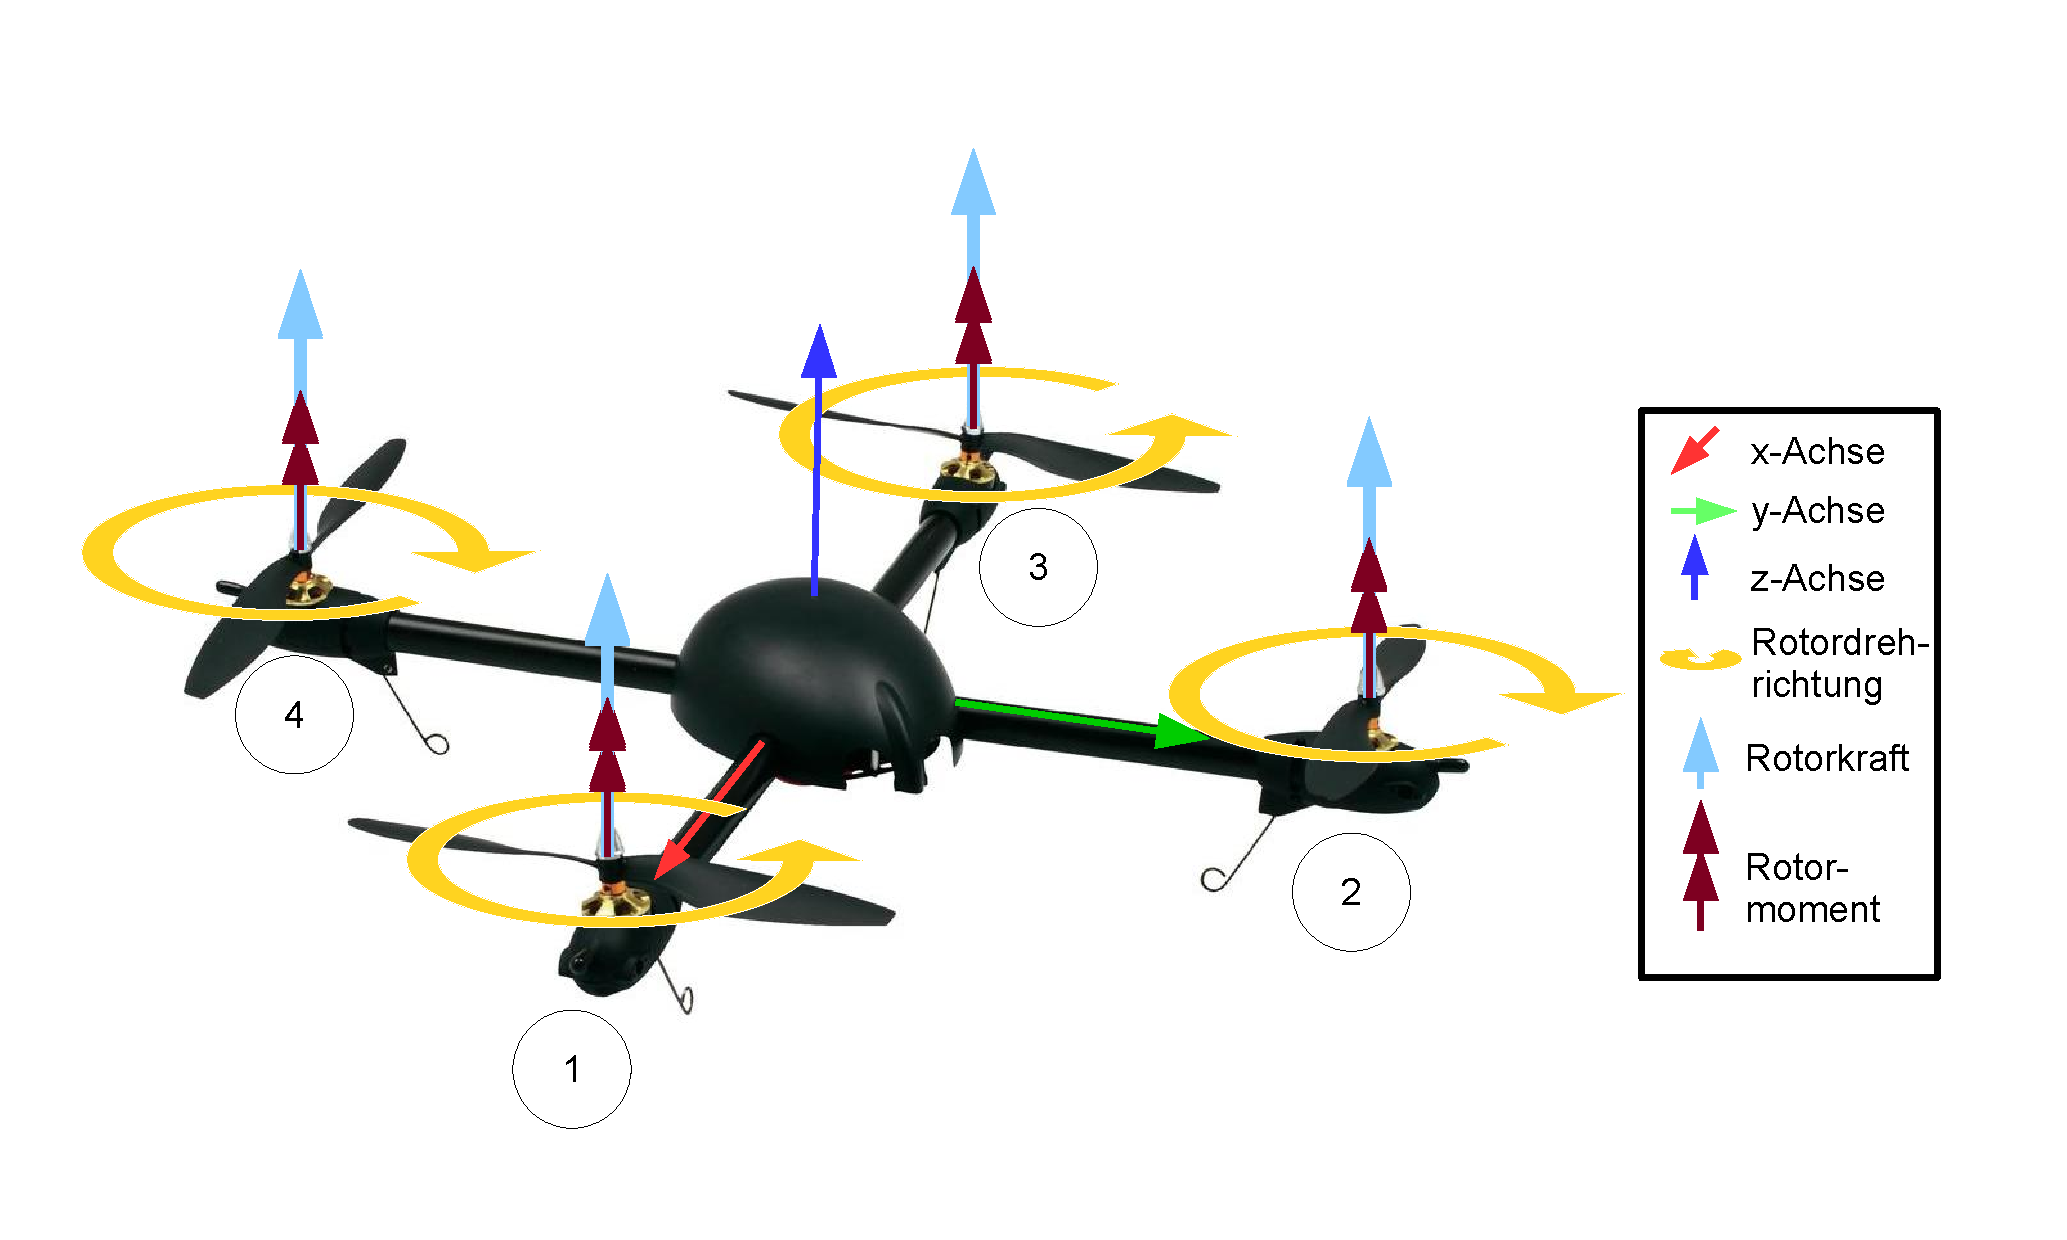
\includegraphics[width = 0.9\textwidth]{images/funktionsweise_quadrocopter}
	\caption[Momente und Kr�fte an einem Quadrocopter]{Momente und Kr�fte an einem Quadrocopter}
	\label{fig:funktionsprinzip}
\end{figure}

\begin{equation}
S^b = \begin{bmatrix}
S^{b}_x\\
S^{b}_y\\
S^{b}_z\\
\end{bmatrix}
=
\begin{bmatrix}
0\\
0\\
F_1+F_2+F_3+F_4\\
\end{bmatrix}
\label{eq:Schubvektor}
\end{equation}

Damit der Qudrocopter eine Bewegung im Raum vollziehen kann, muss dieser Vektor aus der Vertikalen ausgelenkt werden. Dies wird durch eine �nderung der Lage realisiert. Reduziert man zum Beispiel die Drehzahl $n_1$ und erh�ht gleichzeitig die Drehzahl $n_3$ hat das resultierende Kr�fteungleichgewicht �ber die L�nge $ l $ der Quadrocopterarme ein positives Moment um die $y^b$-Achse zur Folge. Der Quadrocopter dreht sich um die $y^b$-Achse, der Pitch-Winkel �ndert sich. Der Quadrocopter erf�hrt in der horizontalen Ebene des Raums eine Beschleunigung. Das gleiche Prinzip gilt auch f�r den Roll-Winkel, sprich Rotation um die $x^b$-Achse. Hier ist allerdings der Drehzahlenunterschied zwischen $n_2$ und $n_4$ verantwortlich f�r die Rotation.

Eine �nderung der Orientierung um die Hochachse z, sprich �nderung des Yaw-Winkels, l�sst sich ebenfalls �ber Variation der Rotordrehzahlen hervorrufen. Dabei kommt der Effekt zum tragen, dass der Widerstand der umgebende Luft entgegen der Drehrichtung der Motoren eine Kraft auf die Rotorbl�tter einpr�gt. Je nach Drehrichtung der Rotoren wirkt damit ein Moment auf den Quadrocopter.
% Somit �ber die Rotoren Momente auf den Quadrocopter wirken.
Diese Momente, die an den Armen des Quadrocopters angreifen, lassen sich zur Vereinfachung in den Schwerpunkt verschieben. Damit bei gleicher Drehzahl aller Rotorbl�tter ein Momentengleichgewicht herrscht, drehen sich die Motoren eins und drei gegen, die Motoren zwei und vier mit dem Uhrzeigersinn. Um die gew�nschte Rotation zu erzielen, wird die Drehzahl $n_1$ und $n_3$ erh�ht und gleichzeitig  $n_2$ und $n_4$  reduziert. Das Ergebnis ist eine Rotation in positive Richtung.

Zusammenfassen lassen sich die f�r die Rotation um die Quadrocopter-Achsen verantwortlichen Momente $M^{b}_{x,y,z}$ in einem Vektor $M^b$ zusammenfassen.  

\begin{equation}
M^b = \begin{bmatrix}
M^{b}_x\\
M^{b}_y\\
M^{b}_z\\
\end{bmatrix}
=
\begin{bmatrix}
l(F_3-F_1)\\
l(F_2-F_4)\\
M_1-M_2+M_3-M_4\\
\end{bmatrix}
\end{equation}

Aufzukl�ren ist, warum mit einer Erh�hung der Drehzahl auch immer eine Reduzierung des Gegenparts verkn�pft ist. Die Begr�ndung lautet, dass der Schubvektor $S^b$ durch eine Rotation m�glichst wenig beeinflusst werden soll.%, um mit der Gesamtschubvorgabe ganz einfach bestimmt zu werden. 


\section{Aufbau der Hardware}
\label{sec:Hardwareaufbau}
Zum Einsatz kommt der AscTec Pelican der Firma \gls{asctec} \cite{hmpgasctec}. Dieser Quadrocopter ist eine spezielle Entwicklung f�r die Forschung. Seine Turmstruktur erm�glicht eine einfache Integration zus�tzlicher Sensoren und Nutzlasten. Durch die Flexibilit�t im Aufbau ist das Ziel dieses Teilkapitels, einen �berblick zur Position der einzelnen Komponenten zu geben. Begleitend zum Text sind diese in Abbildung \ref{fig:hardwareaufbau} dargestellt.\\

	\begin{figure}
		\centering
		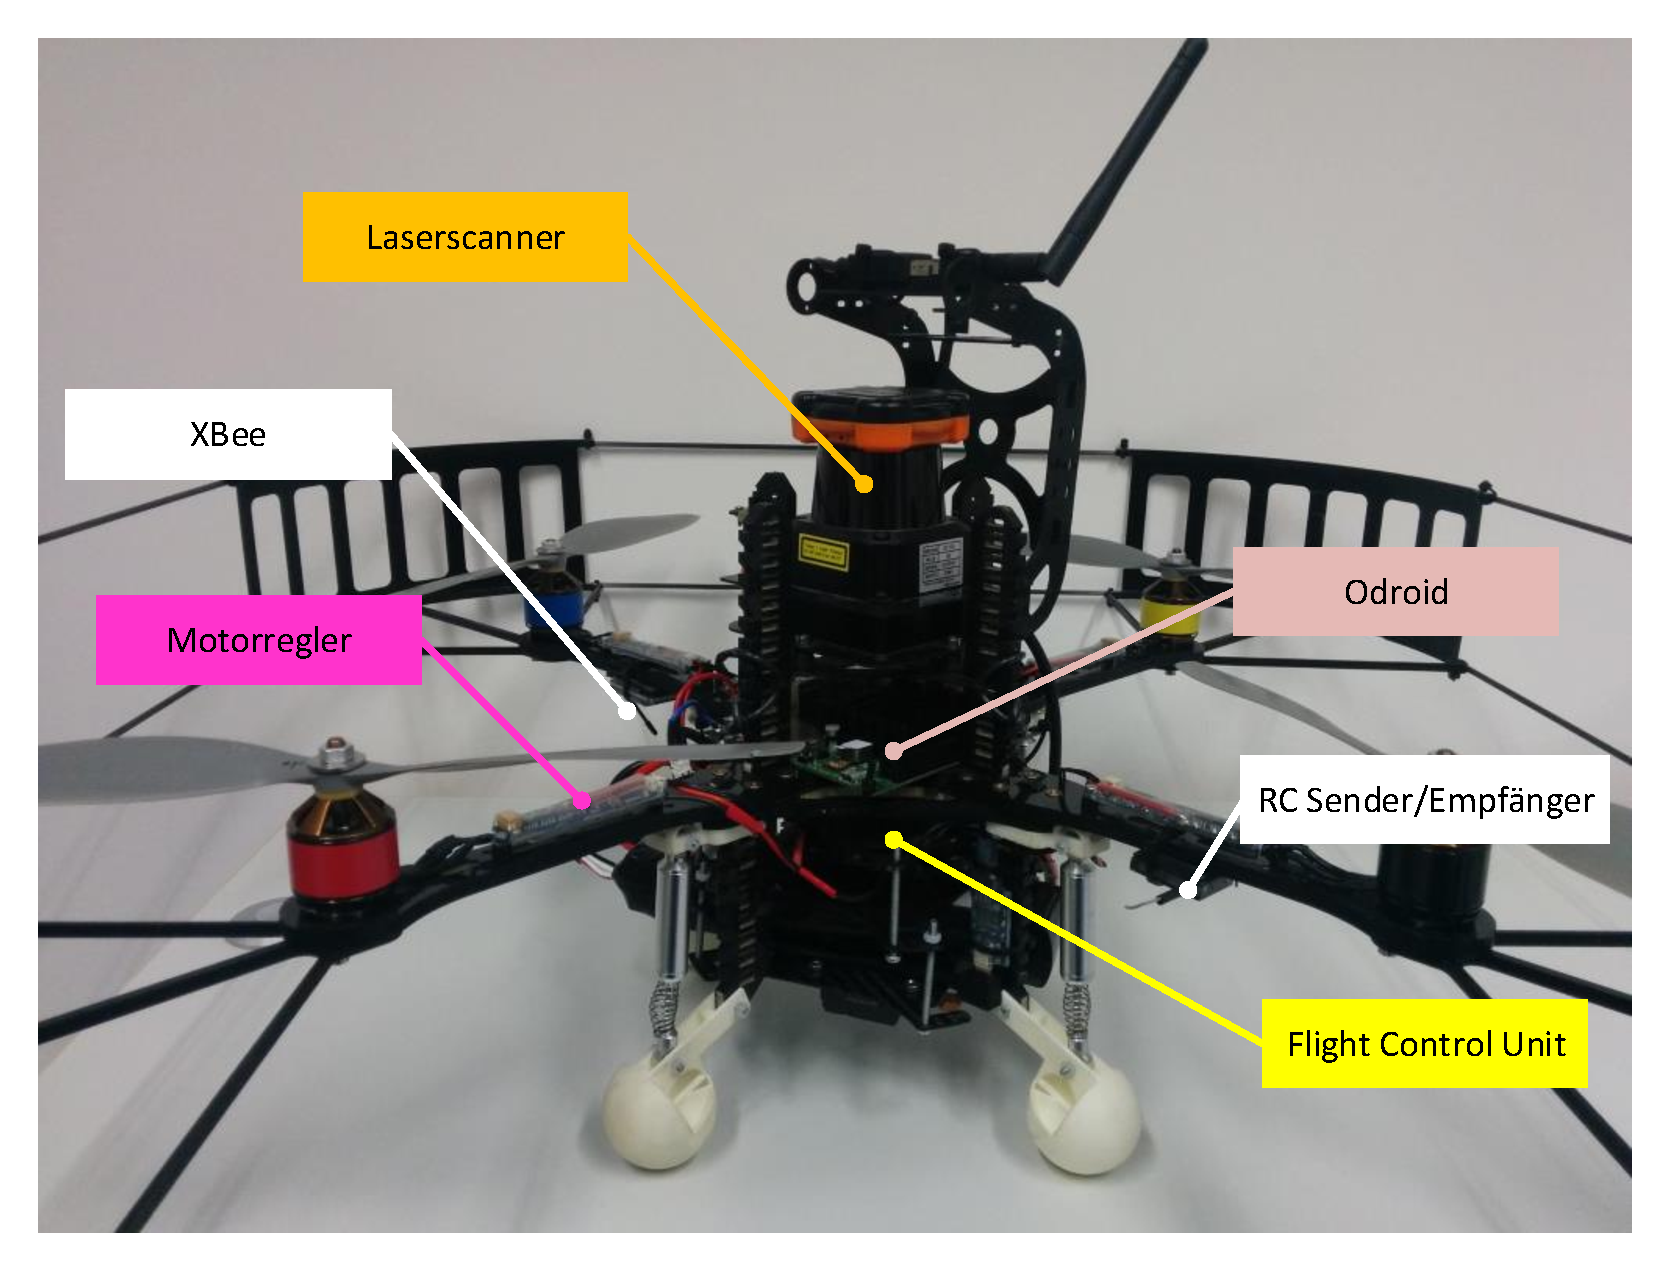
\includegraphics[width = 0.75\textwidth]{images/Hardwareaufbau}
		\caption[Hardwareaufbau des Quadrocopters]{Hardwareaufbau des Quadrocopters}
		\label{fig:hardwareaufbau}
	\end{figure}

F�r jeden der vier mit einem Propeller verbundenen Elektromotoren sind separate Motorcontroller zust�ndig. Diese sorgen daf�r, dass sich die von der \gls{fcu} angeforderten Drehzahlen einstellen.

Die \gls{fcu} ist die zentrale Steuer- und Regeleinheit des Quadrocopters. Sie besitzt zwei ARM7 Prozessoren, einen \gls{llp} und einen \gls{hlp}, zudem verschiedene Kommunikationsschnittstellen (vgl. Kapitel \ref{fig:Kommunikationsstruktur}). Zus�tzlich besitzt \gls{fcu} eine inertiale Messeinheit (engl. \gls{imu}). Diese Einheit wird zur Bewegungsdetektion sowie zur Bestimmung der Lage und Ausrichtung ben�tigt. Sie ist nicht zur Positionsbestimmung in einem ortsfesten Koordinatensystem geeignet. Bestandteile der \gls{imu} sind ein 3D-Beschleunigungssensor, drei Drehratensensoren (Gyros), ein Kompass sowie ein Drucksensor zur Ermittlung der Flugh�he anhand des Luftdrucks. Verbaut sind die Sensoren mit Ausnahme des Kompass direkt auf der Platine (Abbildung \ref{fig:fcuplatien}).

Da der Einsatzbereich im Indoorbereich liegt, ist der Drucksensor zur H�henbestimmung in geschlossenen R�umen nicht geeignet. Er liefert erst ab einer H�he von $ 5~m $ zuverl�ssige Werte. Daher wurde in einer vorangegangen Arbeit von Jan Kallwies \cite{JanKal13} die Hardware um ein Modul zur Messung der H�he im Indoorbereich erweitert. Auf diesem Modul befinden sich zwei Infrarotsensoren f�r den Nahbereich. Beide zusammen decken einen Bereich von $ 4~cm $ bis $ 142~cm $ ab. Erweitert wird der Messbereich durch einen Ultraschallsensor f�r Entfernungen von bis zu $ 5~m $. Aus diesen drei Sensordaten wird �ber einen Extended-Kalman-Filter die Flugh�he bestimmt. Eine genaue Beschreibung dieses Fusionsfilters kann in der Arbeit von Jan Kallwies \cite{JanKal13} nachgelesen werden. Da in der vorliegenden Arbeit die Navigation in der horizontale Ebene den Schwerpunkt darstellt, wird dieses Modul hier nicht weiter behandelt.

	\begin{figure}
		\centering
		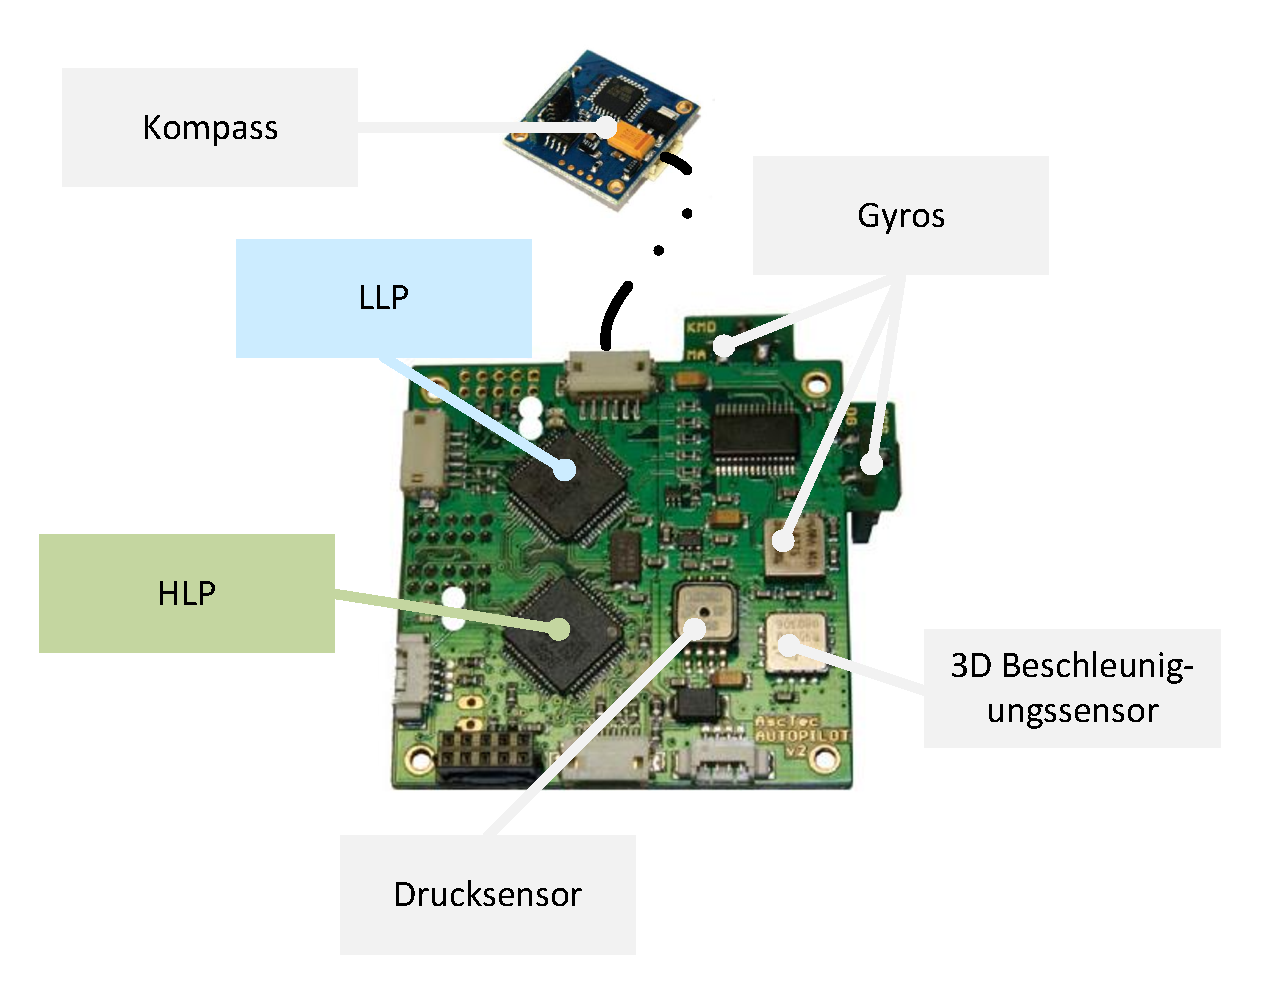
\includegraphics[width = 0.75\textwidth]{images/FCU_Platine}
		\caption[Platine der \gls{fcu}]{Platine der \gls{fcu}}
		\label{fig:fcuplatien}
	\end{figure}
	
Um in der Horizontalen die Navigation zu gew�hrleisten, muss die Position des Flugk�rpers in der xy-Ebene bekannt sein. Da dies, wie schon beschrieben, nicht mit der Inertialsenorik m�glich ist, wurde in die Turmstruktur der Laserscanner UTM-30LX der Firma Hokuyo (Datenblatt Anhang \ref{anh:datasheet}) integriert. Dieser Scanner hat eine maximale Reichweite von $ 30~m $ und ein Abtastbereich von $ 270^\circ $. Die Umlauffrequenz betr�gt dabei $ 40~Hz $, d.h. alle $ 25~ms $ steht ein neuer Scan zur Verf�gung.    

Damit zur Berechnung der Position sowie der Implementierung weiterer Algorithmen und Funktionen ausreichend Rechenleistung zur Verf�gung steht, befindet sich auf dem Quadrocopter ein zus�tzlicher Odroid-X Mikrocomputer mit einem Quad Core Prozessor mit $ 1.4~GHz $ und $ 1024~MB $ LP-DDR2 Arbeitsspeicher. Au�erdem besitzt diese Entwicklungsplattform sechs USB-Schnittstellen sowie einen $ 10/100~Mbps $ Ethernet-Anschluss.\\


%Nach dem �berblick �ber die im Quadrocopter verbaute Hardware und deren Komponenten, geht das folgende Kapitel \ref{sec:Kommunikationsarchitekur} auf die Implementierung der Intelligenz �ber Software ein.

%Nun sollte man einen �berblick �ber die im Quadrocopter verbauten Komponenten besitzen. Wie die Einheiten untereinander vernetzt sind, darauf wird im folgenden Kapitel \ref{sec:Kommunikationsarchitekur} eingegangen.

     
\section{Softwarearchitektur und Kommunikationsstruktur}
\label{sec:Kommunikationsarchitekur}

Nachdem im vorhergegangenen Kapitel \ref{sec:Hardwareaufbau} die verbaute Hardware vorgestellt wurde, geht es in diesem Abschnitt um die Softwarearchitektur (Abbildung \ref{fig:Kommunikationsstruktur}). Es wird aufgezeigt, welche Software bereits fest implementiert ist und wo adaptive Applikationen integriert werden k�nnen. Des Weiteren wird die Kommunikationsstruktur dargelegt, wie und �ber welche Protokolle die einzelnen Komponenten miteinander kommunizieren. \\
\begin{figure}
	\centering
	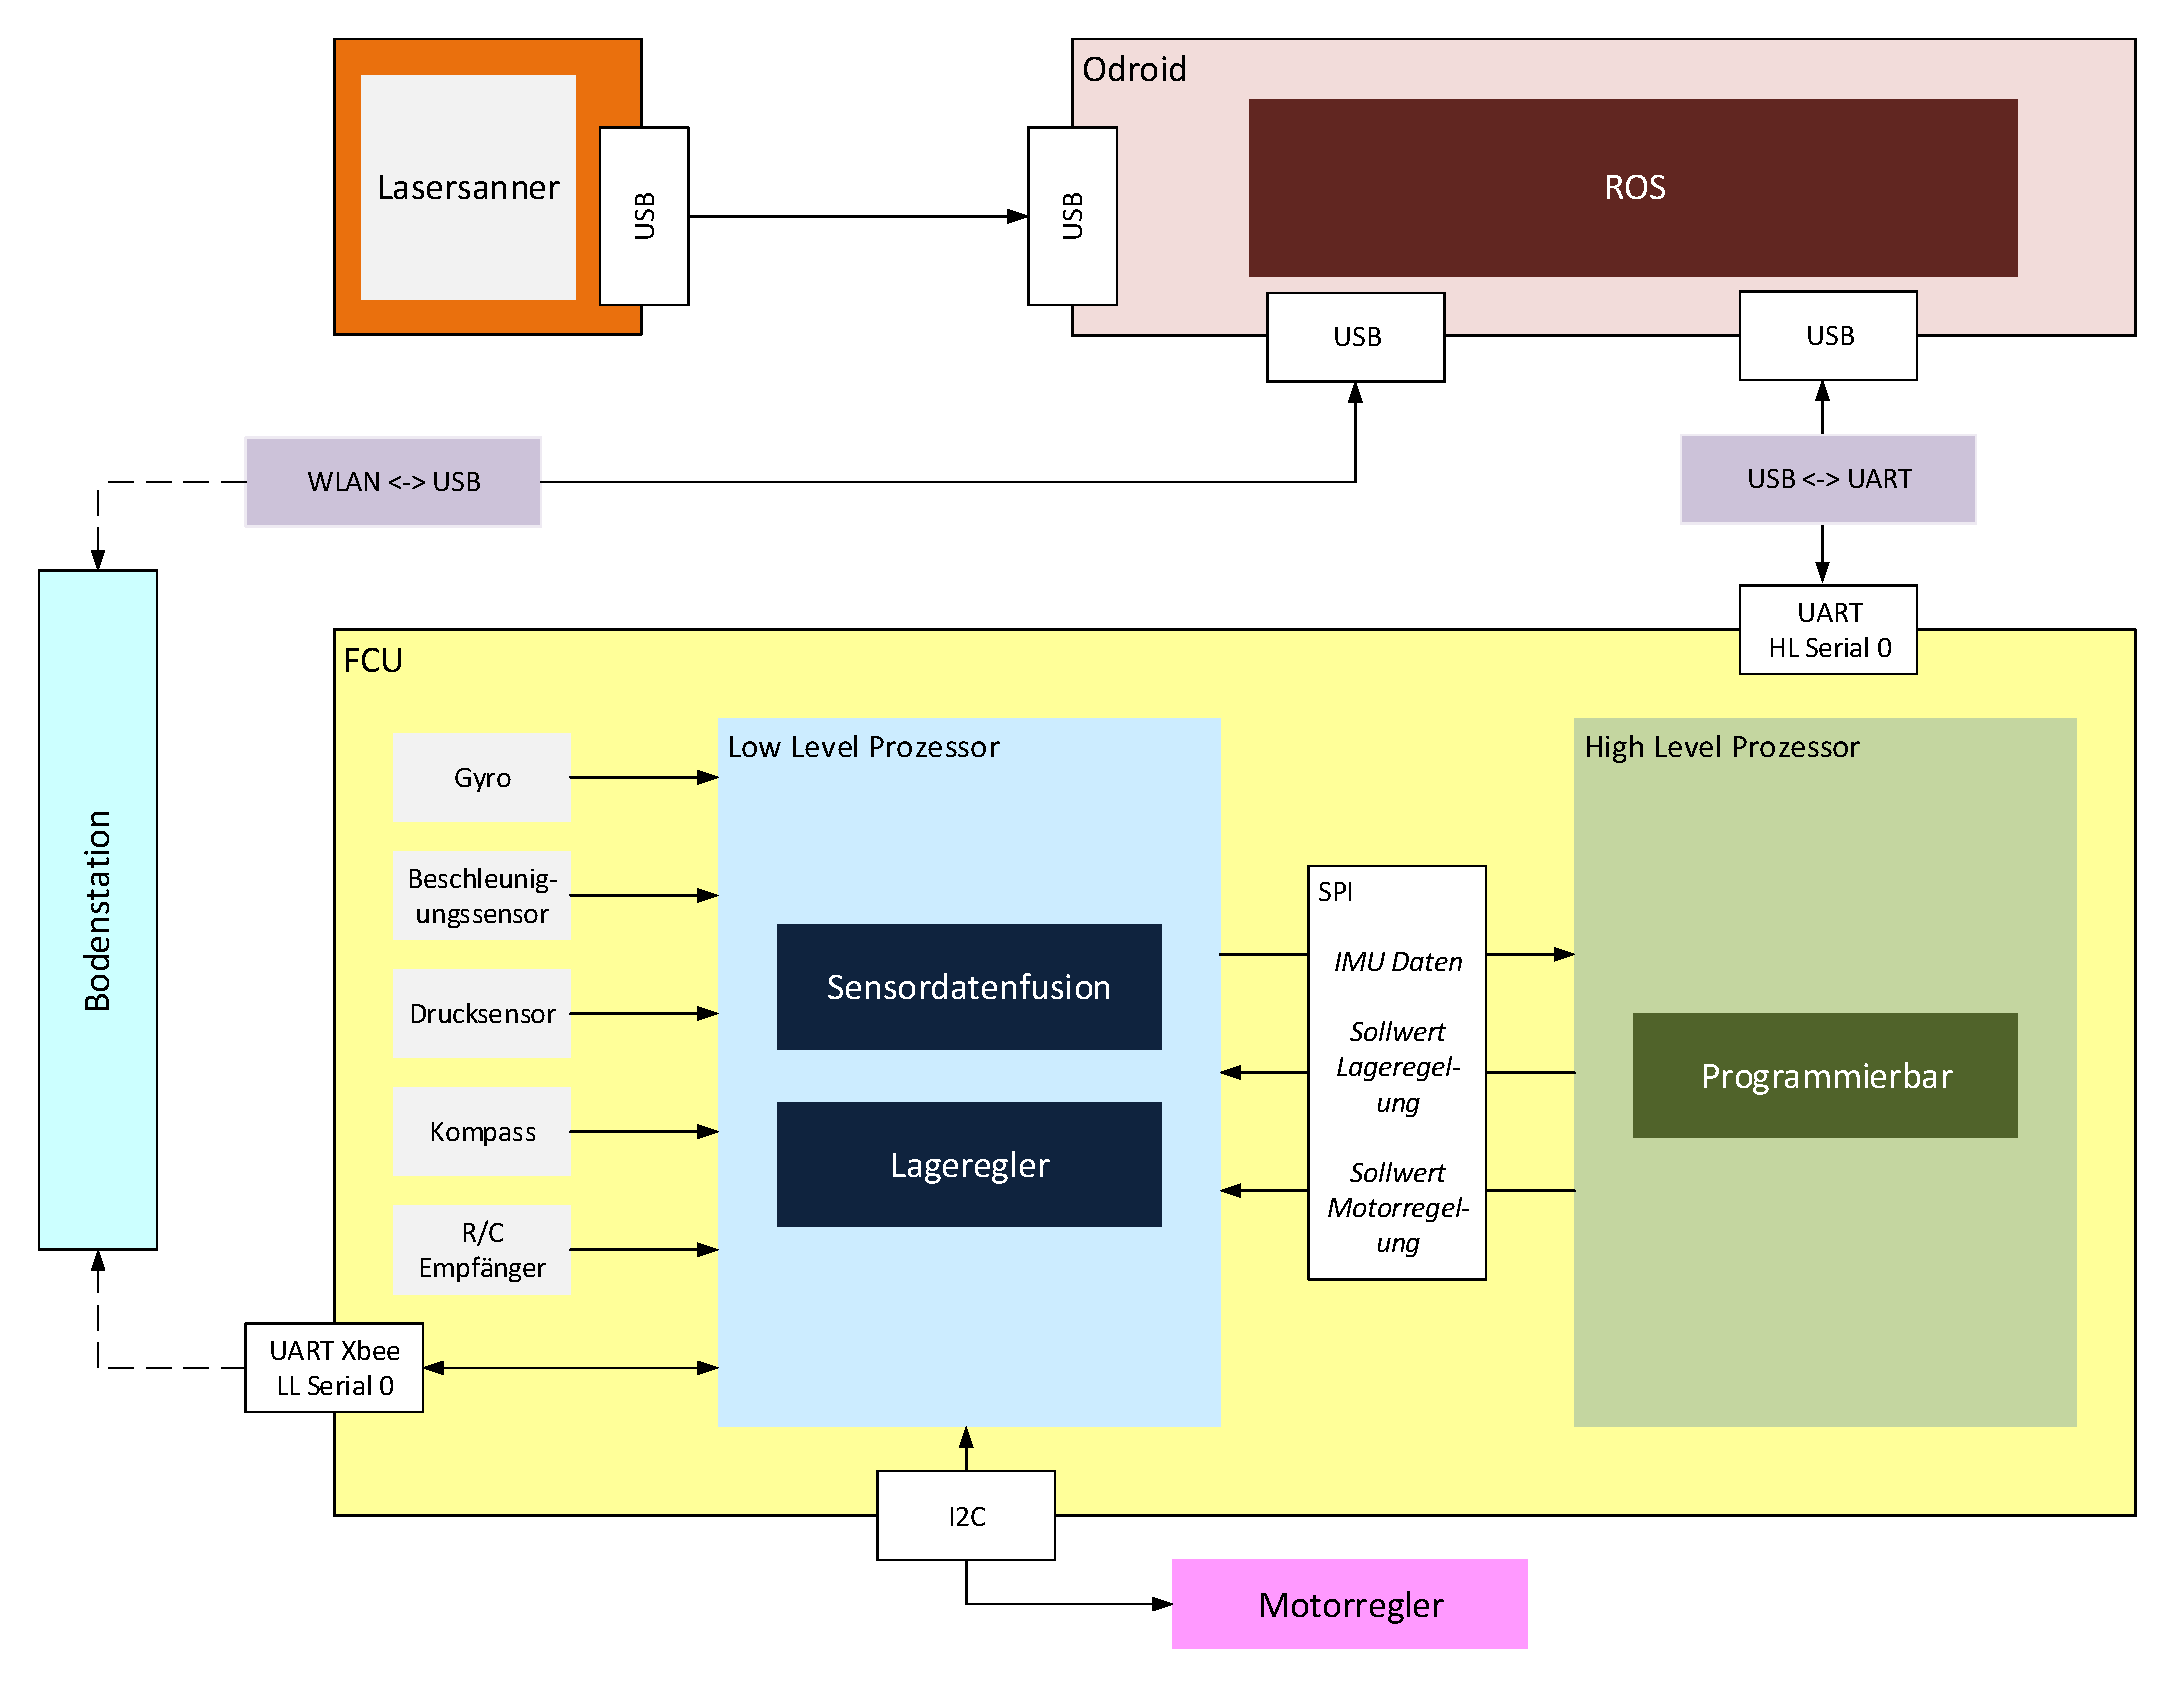
\includegraphics[width = \textwidth]{images/Kommunikationsarchitektur}
	\caption[Softwarearchitektur und Kommunikationsstruktur des Quadrocopters]{Softwarearchitektur und Kommunikationsstruktur des Quadrocopters}
	\label{fig:Kommunikationsstruktur}
\end{figure}
Beginnend mit den beiden Prozessoren 
%der \gls{llp} und \gls{hlp} 
der \gls{fcu}, deren Hauptschleifen der Software mit einer Frequenz von $ 1~kHz $ durchlaufen werden und die 
%mit der \gls{fcu}, deren beiden Prozessoren \gls{llp} und \gls{hlp} mit einer Frequenz von 1kHz getaktet werden und 
�ber einen \gls{spi} Bussystem verkn�pft sind, wird zun�chst der \gls{llp} betrachtet. Auf dem Low Level Prozessor befindet sich die Sensordatenfusion der \gls{imu}-Sensorik zur Lagebestimmung des Quadrocopters. Darauf basiert die Lageregelung, die das Flugverhalten stabilisiert. Hier�ber werden die geforderten Sollwinkel bzw. die Solllage eingestellt, die dem \gls{llp} �ber die Fernbedienung oder den \gls{hlp} �bergeben werden. Kombiniert mit der Schubvorgabe werden den Motorreglern die jeweiligen Solldrehzahlen der Rotoren �ber einen \gls{i2c}-Bus �bergeben. Diese Algorithmen sind fest eingepflegt und gew�hrleisten bei Experimentalfl�gen eine sichere R�ckfallebene. Mit dem \gls{llp} stellt \gls{asctec} dem Benutzer eine Art White-Box zur Verf�gung, d.h. die Integration ist bekannt, jedoch nicht deren Umsetzung. �berwachen l�sst sich der LLP �ber einen externen \gls{pc}, in Abbildung \ref{fig:Kommunikationsstruktur} als Bodenstation bezeichnet. Zur Kommunikation werden zwei XBee Funkmodule ben�tigt. Eines ist am \gls{uart} LL-Serial0 Port der \gls{fcu} angeschlossen, das andere am USB Port der Bodenstation. Mit der AutoPilot Software lassen sich unter anderem der Akkustand, die \gls{imu}-Daten sowie die Stellgr��en der Fernsteuerung betrachten. Au�erdem ist es m�glich, Parameter der Sensorfusion und der Lageregelung auszulesen und zu ver�ndern.


Mit dem \gls{hlp} stellt \gls{asctec} eine Entwicklungsumgebung zur Implementierung eigener Algorithmen auf der \gls{fcu} zur Verf�gung. Hier k�nnen erweiternde Programmteile integriert werden, die den Lageregler des \gls{llp} ansprechen oder die direkt den Motorcontroller �ber den \gls{llp} mit Solldrehzahlen speisen.

Die experimentelle Software auf dem \gls{hlp} kann �ber die Fernbedienung aktiviert und deaktiviert werden. Eine fehlerhafte Programmierung des \gls{hlp} kann kritische Flugman�ver hervorrufen. Damit diese nicht zum Absturz f�hren, kann �ber die Fernbedienung die Experimentalsoftware deaktiviert und das Flugsystem �ber die ausgereifte Lageregelung auf dem \gls{llp} stabilisiert werden (R�ckfallebene).

Wie schon in Kapitel \ref{sec:Hardwareaufbau} beschrieben, befindet sich auf dem Quadorcopter zur Erh�hung der Rechenleistung der Odroid-X. Anders als bei den auf der \gls{fcu} befindlichen Prozessoren, besitzt das Odroid-Bord ein Betriebssystem. Es handelt sich dabei um das opensource Betriebssystem Ubuntu 13.04. Dieses wurde ausgew�hlt, da es die Installation eines weiteren opensource Betriebssystems erm�glicht, dem \gls{ros}, einem Software Framework f�r Roboteranwendungen (Kapitel \ref{sec:ros}). Zum Einsatz kommt der Odroid-X bei der Implementierung der Positionsbestimmung (Kapitel \ref{chap:2Dpositionsbestimmung}). Verbunden ist es zum einen �ber einen USB-Port mit dem Laserscanner. Zum anderen mittels eines weiteren USB-Port �ber einen \gls{ftdi}-Konverter am HL-Serial0 Port des \gls{hlp} angeschlossen.
Von der Bodenstation kann �ber \gls{wlan} eine \gls{ssh}~-~Verbindung aufgebaut werden, die in Folge die Entwicklungsplattform bedient.

Nun ist bekannt, wie die einzelnen Komponenten untereinander vernetzt sind. Im weiteren Verlauf der Arbeit l�sst sich nachvollziehen, an welchen Stellen die Anwendungen implementiert werden und �ber welche Verbindungen sie miteinander kommunizieren. 


\chapter{Grundlagen}
\label{chap:grundlagen}
Das Kapitel Grundlagen behandelt die Themen, die in mehreren Abschnitten dieser Arbeit relevant sind. Dabei handelt es sich um das Robot Operation System, die verwendeten Koordinatensysteme und die Transformation zwischen ihnen.

\section{Das Robot Operation System \gls{ros}}
\label{sec:ros}
Ziel dieses Unterkapitel ist es das Opensource Betriebssystem \gls{ros} vorzustellen. Wie es aufgebaut ist und welche Vorz�ge es besitzt.\\

\gls{ros} stellt dem Softwareentwickler Bibliotheken und Werkzeuge zur Verf�gung, die Helfen Roboteranwendungen zu erstellen. Das auf einem \gls{ip}-basierende  modulare Kommunikationsframework erm�glicht die Verkn�pfung von Anwendungssoftware, Sensoren und Aktoren sogar unter mehreren Robotern. Die Grundlage daf�r ist die sogenannte Hardwareabstraktion. Dabei wird durch hardwarespezifische Module erreicht, das Komponenten unterschiedlicher Hersteller miteinander verbunden werden k�nnen. In unserem Fall Hokuyo Lasersanner und \gls{asctec} \gls{fcu}. Au�erdem erm�glicht es eine hardwareunabh�ngige Programmierung, die  in den Programmiersprachen C/C++ oder in Python erfolgen kann. Jede Hardwareabstraktion oder Anwendung wird als Node, bzw. Konten bezeichnet und l�uft als eigener Prozess.
\begin{figure}
	\centering
	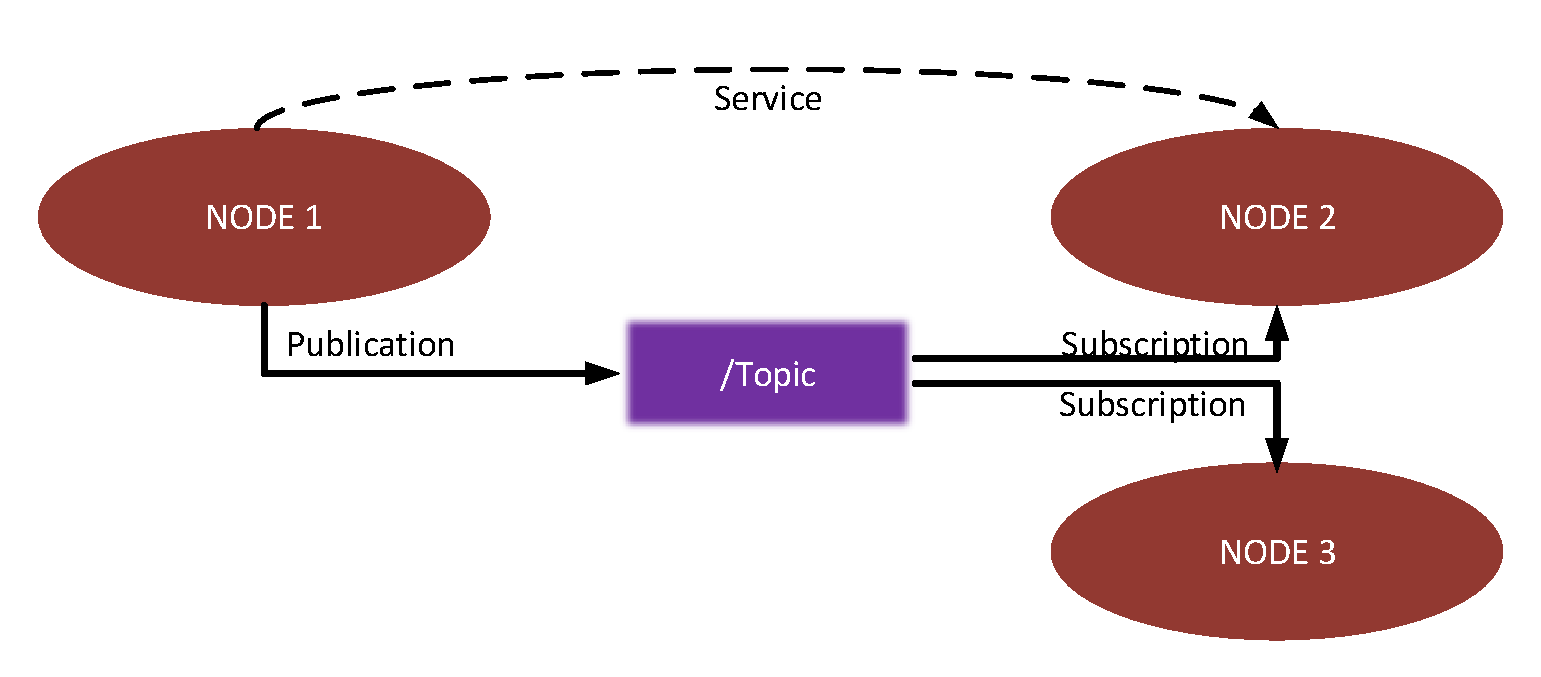
\includegraphics[width = 0.75\textwidth]{images/TopicUndService}
	\caption[Topic und Service]{Kommunikation von Nodes �ber Topics und Services}
	\label{fig:node_kommunikation}
\end{figure}


Der Austausch von Daten zwischen den Nodes erfolgt �ber so genannte Topics (Abbildung \ref{fig:node_kommunikation}]. Dabei werden von den Knoten Nachrichten (engl. Messages) in Topics gepostet und somit ver�ffentlicht (publication). Ben�tigt ein weiter Knoten den Inhalt dieses Topic kann er es abonnieren (subscription). Sobald die Nachricht im Knoten aktualisiert wurde, wird sie den abonnierenden Knoten �bertragen. Dabei sind Knoten nicht auf ein Topic beschr�nkt, es k�nnen beliebig viele Topics beschrieben oder empfangen werden. Alternative zu dieser Art der asynchronen Daten�bertragung, biete \gls{ros} die M�glichkeit einer Synchrone Kommunikation zwischen zwei Nodes �ber Services. Dabei wird auf einem Knoten ein Service gestartet. Dieser dient als Server und agiert nach dem Anfrage-Antwort-Prinzip. Schickt ein anderer Knoten eine Anfrage, wird ihm die geforderte Nachricht zu gesendet. 

Anzumerken ist, das durch das verwendete \gls{ip}-Protokoll keine deterministische Versendung der Nachrichten nicht gew�hrleistet ist, da es sein kann, das Nachrichten gleichen Types in Paketen zusammengefasst werden. Bei der Programmierung empfiehlt es sich daher auf Topics mit einem Zeitstempel (engl. timestamp) zur�ckzugreifen. Die Echtzeitf�higkeit des \gls{ros} ist durch allerdings nicht gef�hrdet. 

\begin{figure}
	\centering
	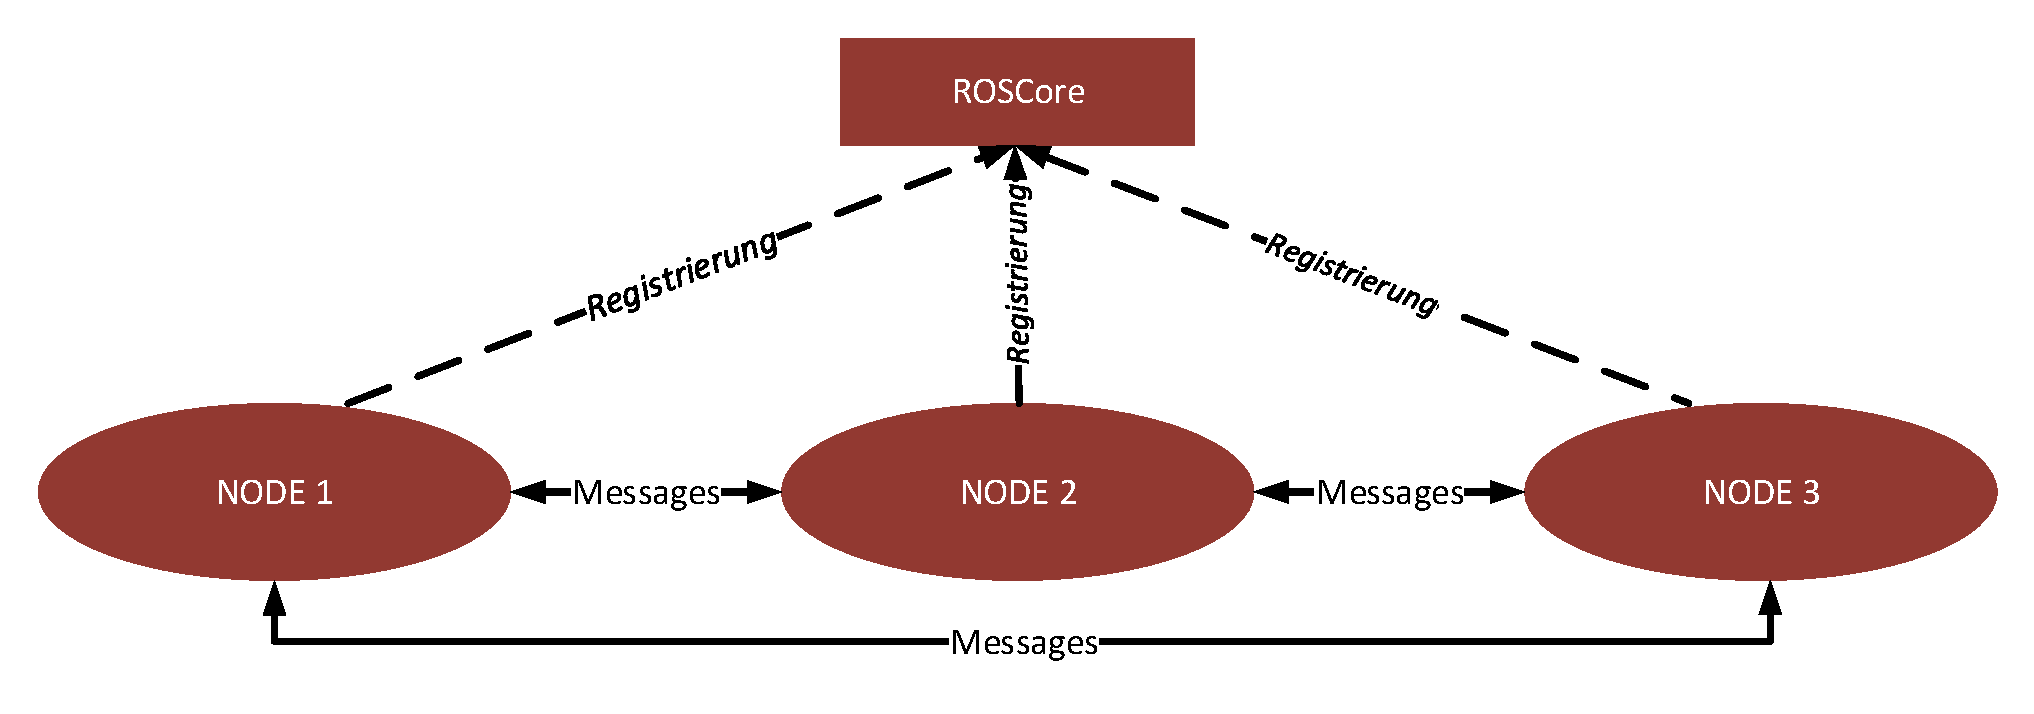
\includegraphics[width = \textwidth]{images/MasterAndNode}
	\caption[Registrierung der Knoten]{Registrierung der Knoten}
	\label{fig:node_master}
\end{figure}


Der wohl gr��te Vorteil von \gls{ros} ist die st�ndig wachsende Community. So stellen Forscher aus der ganze Welt ihre Algorithmen und Hardwareabstraktionen zur Verf�gung. Dadurch ist es m�glich bei der Erstellung einer Roboteranwendung auf Bausteine zur�ck zugreifen, die ohne diese Plattform selbst zu implementieren w�ren. Abgesehen davon stellt ROS eine Vielzahl von Hilfsmitteln wie zum Beispiel die Transferfunktion (/tf) bereit. Hier lassen sich Koordinatensysteme definieren. Die Transformation der Daten wird dann automatisch von \gls{ros} durchgef�hrt.

\section{Einf�hrung in die Koordinatensysteme und Koordinatentransformationen}
\label{sec:koordinatensysteme&transformationen}
Anhand von Koordinatensystemen und Transformationen l�sst sich die Lage von Punkten und  Objekten in einen Raum mathematisch beschreiben. Die Grundvoraussetzung zur Bestimmung der Position des Quadrocopters im 2D-Raum (siehe Kapitel HIER MUSS NOCH EINE REFERENZ HIN). Au�erdem erm�glicht die Einf�hrung von Koordinatensystemen die mathematisch/physikalische Beschreibung des Quadrocopters und stellt somit die Grundlage zur Modellbildung und Reglerentwurf (siehe Kapitel so und so).  

\subsection{Koordinatensysteme}
\label{subsec:koordinatensysteme}
�ber ein Koordinatensystem l�sst sich ein Vektor oder die Position eines Punktes bezogen auf den Koordinatenursprung in einer zweidimensionalen Ebene, bzw in einem dreidimensionalen Raum beschreiben. Ziel diese Teilabschnittes ist die Erl�uterung der in dieser Arbeit eingef�hrten Koordinatensysteme.\\

\begin{figure}
	
	\centering{
		\subfloat[ENU-Koordinatensystem]{
			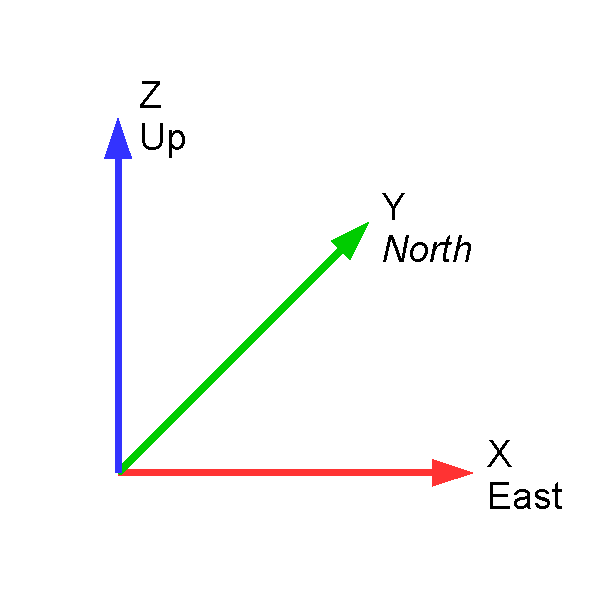
\includegraphics[width=0.3\textwidth]{images/ENU-koordinatensystem}
			\label{fig:enu}
		}
		\subfloat[NED-Koordimatemsystem]{
			\includegraphics[width=0.3\textwidth]{images/ned-koordinatensystem}
			\label{fig:ned}
		}
	}
	\caption[Kovention ]{test}
	\label{fig:konventionen}
	
\end{figure}

Zu Beginn werden nun zwei Konventionen bez�glich der Bezugssysteme vorgestellt. Nummer eins, die in Abbildung \ref{fig:enu} dargestellte \gls{enu} Konvention. Diese wird in vor allem bei der Landnavigation eingesetzt. Hier zeigt die z-Achse nach oben. Bei der zweiten Konvention, haupts�chlich in der Wasser-, Luft- und Raumfahrt eingesetzt, handelt es sich um das \gls{ned} Bezugssystem (Abbildung \ref{fig:ned}). Die z-Achse zeigt nach unten. Anzumerken ist, das in dieser Arbeit die Ausrichtung der x- und y -Achse nicht wie in Abbildung \ref{fig:konventionen} und auch der Namensgebung entsprechend den Himmelsrichtungen entspricht. Die Begriffe \gls{enu} und \gls{ned} dienen hier zur Beschreibung der Ausrichtung der Koordinatenachsen in Abh�ngigkeit der positiven z-Achse.

Bei der nun folgenden Einf�hrung der Koordinatensysteme (Abbildung \ref{fig:koordinatensysteme}) handelt es ausschlie�lich um kartesische, das hei�t orthogonale Koordinatensysteme, die nach der \gls{enu} Konvention ausgerichtet sind. Dies steht erstmal im Widerspruch mit dem Abschnitt zuvor, dort ist das \gls{ned} als Koordinatensystem f�r Flugk�rper eingef�hrt worden. Es ist allerdings so, dass die \gls{ros} Koordinatensysteme auf \gls{enu} basieren. Deshalb die Wahl von Bezugssystemen mit positiver z-Achse nach oben.

\begin{figure}
	\centering
	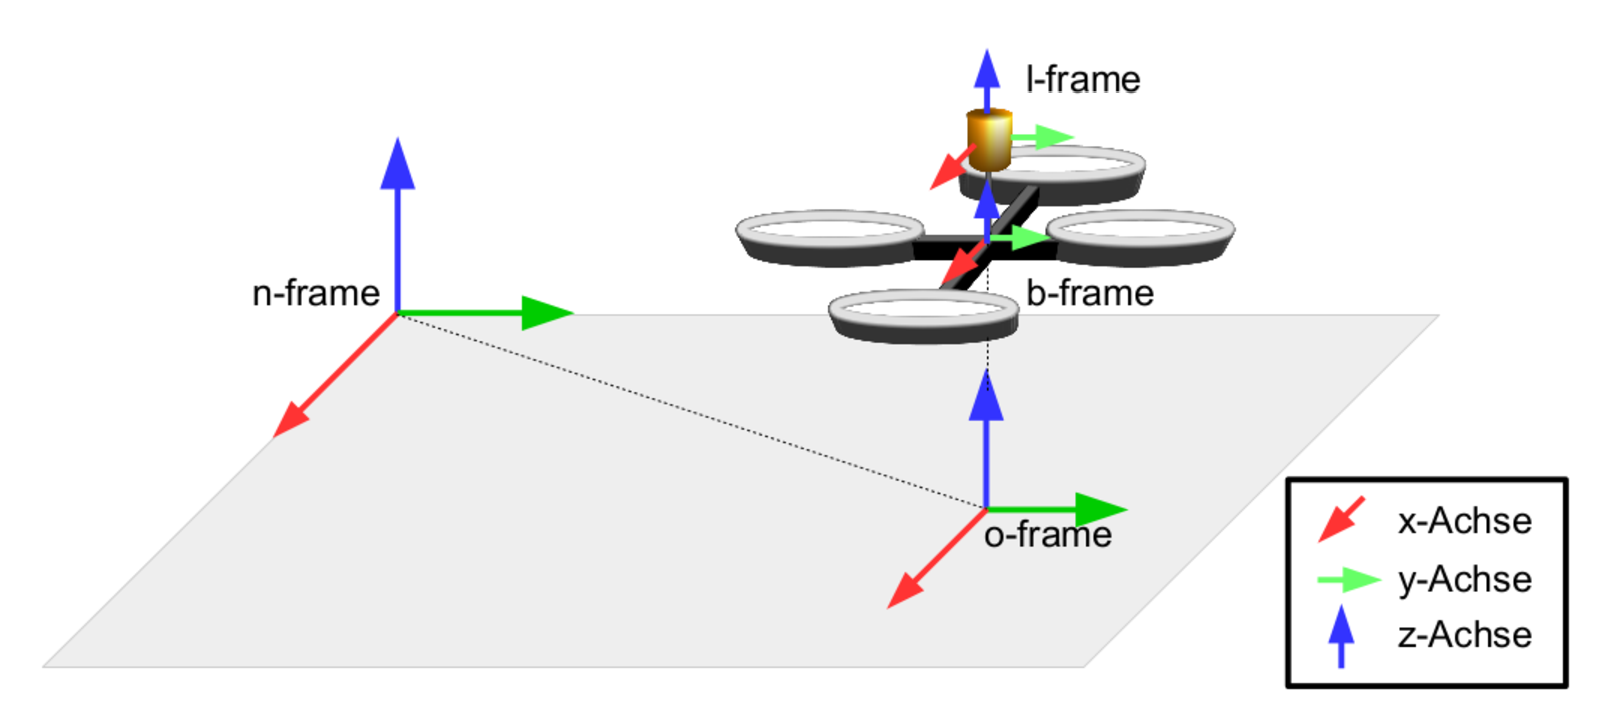
\includegraphics[width = \textwidth]{images/Koordinatensysteme}
	\caption[Koordinatensysteme]{In der Arbeit angewandte Koordinatensysteme }
	\label{fig:koordinatensysteme}
\end{figure}

Wie aus Abbildung \ref{fig:koordinatensysteme} zu entnehmen sind vier xyz-Koordinatensysteme definiert. 

\begin{itemize}
	\item \textbf{n-frame(Lokaler Navigationsframe):} Ortsfestes Koordinatensystem zur Beschreibung der Position im Raum. Da es in dieser Arbeit um die horizontale Positionsregelung geht, ist hier ausschlie�lich die xy-Ebene von Interesse. Der Ursprung des Koordinatensystem wird bei jedem Systemstart neu initialisiert. Zu beachten ist dies beim vollautonomen Flug in R�umen, dabei beziehen sich die Sollpositionen nicht auf ein Raumkoordinatensystem mit festem Ursprung, sondern auf den beim Systemstart initialsierten Bezugspunkt. Keinen Einfluss hat diese Tatsache auf die Geschwindigkeitsregelung per Fernsteuerung, da hier die relative Bewegung von Interesse ist.
	
	Es sei darauf hingewiesen, dass die Verwendung eines xyz Navigationsframes die Kr�mmung der Erdoberfl�che vernachl�ssigt. Diese ist legitim, da die Drohne in Geb�uden zum Einsatz kommt. M�chte man jedoch Weltweit navigieren, ben�tigt man ein  
	rotationsellipsische Koordinatensysteme[THIELECKE LITVERWEIS]

	\item \textbf{b-frame(Bodyframe):} Dieses Koordinatensystem ist fest mit dem Rahmen des Quadrocopters verbunden. Man spricht dabei von einen k�rperfesten Koordinatensystem. Dabei befindet sich der Ursprung des Systems im Schwerpunkt, die x-Achse zeigt in die als Vorne definierte Richtung. Die y- und z-Achse sind abh�ngig davon nach der \gls{enu} Konvention angeordnet. Informationen die sich auf dieses Referenzsystem beziehen sind unter anderen die \gls{imu}-Daten. Au�erdem l�sst sich mit diesem System die Lage des Quadrocoters im n-frame �ber die Position des Nullpunkts und Drehwinkel beschreiben. 
	 	
	\item \textbf{l-frame(laserframe):} Ebenfalls ein k�rperfestes Koordinatensystem. In die dem Entfernungsmessungen des Lasers aufgetragen werden. Der Bezugspunkt liegt dabei in der Sendequelle des Lasers. Die Ausrichtung der Achsen entspricht der des b-frames, mit Ausnahme eines Offsets in z-Richtung.
	
	\item \textbf{o-frame(Orthogonalframe):} Hierbei handelt es sich um ein objektbezogenes Bezugssystem, dessen Orientierung um seine z-Achse und die Position des Ursprungs im n-frame abh�ngig von dem Orthogonal �ber der Ebene befindlichen b-frame ist. Dadurch wird der Quadrocopter in der zu Navigierenden xy-Ebene abgebildet.  
	
	 \end{itemize}
 
Da sich Messwerte wie zum Beispiel die \gls{imu}-Daten oder die Laserdaten auf unterschiedlichen Koordinatensysteme beziehen, ben�tigt man Koordinatentransformation(Kapitel \ref{subsec:koordinatentransformation}). Mit Hilfe derer lassen sich die Vektoren und Koordinaten in die verschiedenen Bezugssysteme �bertragen.

 
\subsection{Koordinatentransformationen}
\label{subsec:koordinatentransformation}
Damit Daten eines Referenzsystem in einen anderes Transformiert werden k�nnen, muss deren Orientierung zueinander beschreibbar sein. Nach  [Buchholz Flugregelung] ist dies �ber die Rotationswinkel $\phi$ (Rollwinkel/engl. roll), Rotation um die x-Achse sowie der Winkel $\theta$ (Nickwinkel/engl. pitch) und $\psi$ (Gierwinkel/engl. yaw) f�r die y- und z-Achse m�glich. Die Reihenfolge um die die Achsen gedreht werden, ist dabei nicht beliebig. Sie ist in verschiedenen Konventionen festgelegt. In dieser Arbeit wird die in der Luftfahrt- und Fahrzeugtechnik gebr�uchliche z,y',x''- Konvention (Abbildung \ref{fig:zyx_konvention}) angewendet.   

\begin{figure}
	\centering
	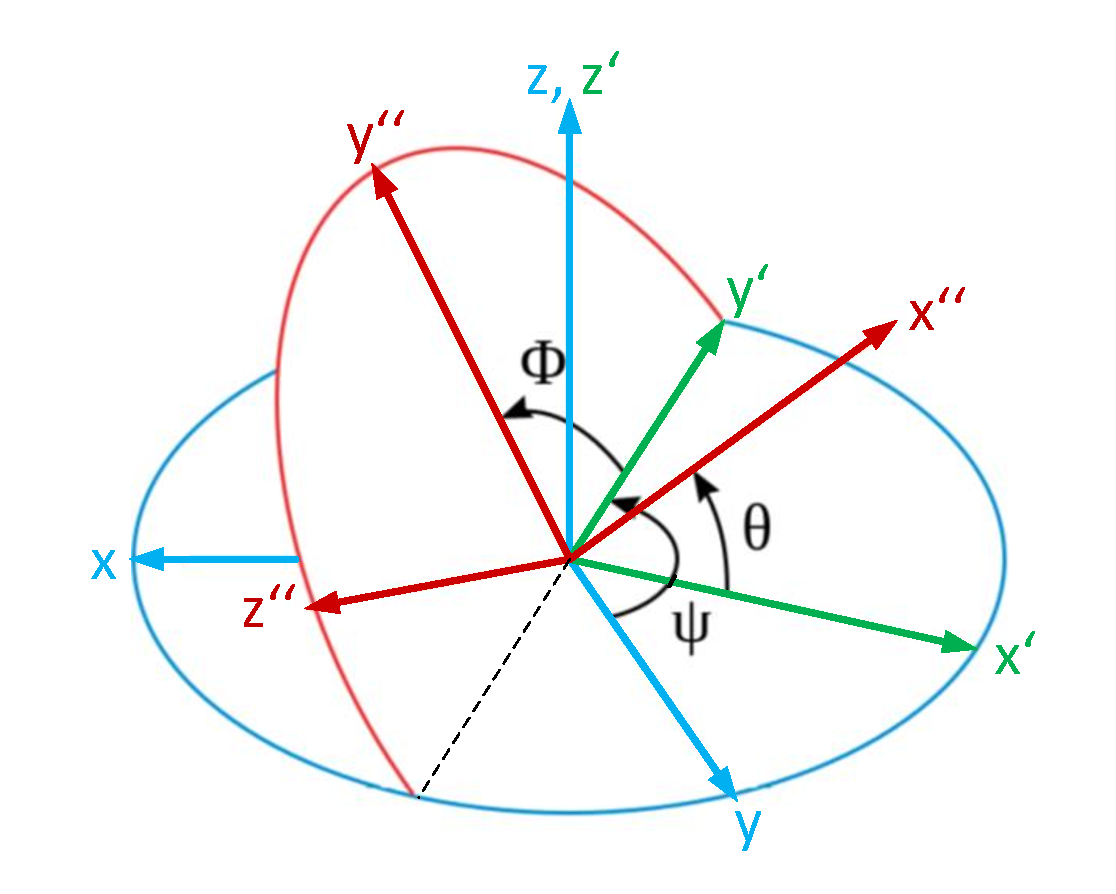
\includegraphics[width = .75\textwidth]{images/zyx_konvention}
	\caption[z,y',x''-Konvention]{z,y',x''-Konvention}
	\label{fig:zyx_konvention}
\end{figure}

Das Koordinatensystem wird zu beginn um den Winkel $\psi$, d.h. um die z-Achse gedreht. Daraus ergibt sich das in Abbildung \ref{fig:zyx_konvention} gr�n eingezeichnet Koordinatensystem. Dieses rotiert man anschlie�end um die Achse y', sprich den Winkel $\theta$. Zuletzt erfolgt eine Drehung mit dem Winkel $\phi$ um die x''-Achse. Das Ergebnis ist das rote x'',y'',z''-Koordinatensystem. Es sein nochmal darauf hinzuweisen, das die Reihenfolge der Winkel einzuhalten ist, da sonst die beschriebene von der tats�chlichen Lage abweicht. Ein veranschaulichendes Beispiel worin unterschiedliche Abfolgen bei der Rotation f�hren ist in der Literatur [Literaturverzeichnis] von Herr Thielecke zu finden.  

Nach Luftfahrtkonvention l�sst sich eine Transformationsmatrix $M$ aufstellen, mit der Vektoren und Koordinaten vom xyz-Koordinatensystem (Bsp.: n-frame) in das x''y''z''-Koordinatensystem (Bsp.: b-frame) �berf�hren lassen. Daf�r ben�tigt man zun�chst die drei Transformationsmatrizen, die jeweils eine Rotation um eine Koordinatenachse beschreiben[Literaturverzeichnis]. Diese sind wie folgt definiert:

\begin{itemize}
	\item Drehung um die z-Achse mit dem Winkel $\psi$
	\begin{equation}
		M_z = \begin{bmatrix}
		\cos\psi 	& -\sin\psi	& 0\\
		\sin\psi	& \cos\psi	& 0\\
		0			& 0 		& 1\\
		\end{bmatrix}
		\label{eq:Mz}
	\end{equation}
	\item Drehung um die y-Achse mit dem Winkel $\theta$
	\begin{equation}
	M_y = \begin{bmatrix}
	\cos\theta  & 0	& \sin\theta\\
	0			& 1	& 0\\
	-\sin\theta	& 0 & \cos\theta\\
	\end{bmatrix}
	\end{equation}
	\item Drehung um die x-Achse mit dem Winkel $\phi$
	\begin{equation}
	M_x = \begin{bmatrix}
	1	& 0			& 0\\
	0	& \cos\phi	& -\sin\phi\\
	0	& \sin\phi 	& \cos\phi\\
	\end{bmatrix}
	\end{equation}
\end{itemize}

Aus diesen Rotationsmatrizen l�sst sich �ber Matrizenmultiplikation eine Gesamttransformationsmatrix aufstellen. Die Reihenfolge der Multiplikation entspricht der in der Konvention festgelegten Drehfolge, von rechts nach links gelesen. Somit er gibt sich:

	\begin{equation}
	\begin{split}
	M_{bn} &	= M_x \cdot M_y \cdot M_z \\
	&= \begin{bmatrix}
	\cos\theta\cos\psi	& \cos\theta\sin\psi	& -sin\theta\\
	\sin\phi\sin\theta\cos\psi-\cos\phi\sin\psi	& \sin\phi\sin\theta\sin\psi+\cos\phi\cos\psi	& \sin\phi\cos\theta\\
	\cos\phi\sin\theta\cos\psi+\sin\phi\sin\psi	& \cos\phi\sin\theta\sin\psi-\sin\phi\cos\psi 	& \cos\phi\cos\theta\\
	\end{bmatrix}
	\end{split}
	\end{equation}
FORMEL �BERPR�FEN DA FEHLER IN ROATIONSMATRIZEN GEFUNDEN. DIESE SIND BEREITS BEHOBEN. NERNEUT �BERPR�FEN. WAR VORHER WAHRSCHEINLICH DOCH RICHTIG IN Gleichung POSE BESTIMMUNG HANDELT ES SICH IM EINE INVERSER ALSO TRANSFORMIERTE FORM VON MZ!!!!!!!!! Mz My Mx WAHRSCHEINLICH FALSCH SO WIE SIE DA STEHEN.
Mit Hilfe dieser Transformationmatrix l�sst sich jetzt ein Vektor zum Beispiel aus dem n-frame ins b-frame �bertragen.

\begin{equation}
\begin{bmatrix}
x^b\\
y^b\\
z^b\\	
\end{bmatrix} = M_{bn} \cdot 
\begin{bmatrix}
x^n\\
y^n\\
z^n\\	
\end{bmatrix}
\label{eq:inverse_transM} 
\end{equation}

Handelt es sich bei um eine Koordinate, ist zus�tzlich noch der Abstand der Koordinatenurspr�nge zu addieren. F�r die R�cktransformation muss die Gesamttransformationsmatrix transponiert werden. Daraus folgt,

   \begin{equation}
   \begin{bmatrix}
   x^n\\
   y^n\\
   z^n\\	
   \end{bmatrix} = M_{bn}^T \cdot 
   \begin{bmatrix}
   x^b\\
   y^b\\
   z^b\\	
   \end{bmatrix} = M_{nb} \cdot 
   \begin{bmatrix}
   x^b\\
   y^b\\
   z^b\\	
   \end{bmatrix}
   \label{eq:inverse_transM}
   \end{equation}

Nun lassen sich Vektoren in beide Richtungen in die verschiedenen Bezugssysteme �berf�hren. Nachteil der Methode mit Eulerwinkel ist, das diese auf Grund der trigonometrischen Funktionen nur f�r Winkel $\phi, \theta, \psi = \{x \in  \mathbb{R}| -\pi \le x \le \pi\}$ eindeutig durchf�hrbar ist. Wird dieser Bereich �berschritten, l�sst sich die Lage �ber Quaternionen beschreiben. Durch die Beschreibung der dreidimensionalen Orientierung in einem vierdimensionalen Raum lassen, ist die Lage auch f�r Rotationen um eine vielfaches von $2\pi$ eindeutig charakterisiert. Die genaue Definition findet sich in der  Literatur [THIELECKE] und [YOUTUBE]. Da die Definitionsbereich der Eulerwinkel f�r den in der Arbeit betrachteten Bereich ausreicht ist ausschlie�lich die Umrechnung der in Quaternion ($w_q$, $x_q$, $y_q$, $z_q$) angegebenen Orientierungsdaten der \gls{imu} in Eulerwinkel($\phi$, $\theta$, $\psi$). Zu beachten ist, das die nun folgende Umwandlung nur f�r die $z,y',x''$-Konvention G�ltigkeit besitzt. 
  
   \begin{equation}
	   \phi = \arctan(\frac{2(y_qz_q+w_qx_q)}{w_q^2-x_q^2-y_q^2+z_q^2})\\
	\end{equation}
   \begin{equation}
	  \theta =\arcsin(2(w_q y_q -x_q z_q))\\
   \end{equation}
   \begin{equation}
     \psi = \arctan(\frac{2(x_q y_q + w_q z_q)}{w_q^2+x_q^2-y_q^2-z_q^2})
   \end{equation}
 
 Mit dieser letzten Umrechnung sind alle Grundlagen f�r die Arbeit gelegt. So bilden die Koordinatensystem und Transformationen die Basis f�r die nachkommende Positionsbestimmung. 



\printglossary[style=altlist,title=Glossar]

% Anhang (Bibliographie darf im deutschen nicht in den Anhang!)
\bibliography{bib/BibtexDatabase}
\clearpage
%\addcontentsline{toc}{chapter}{Abbildungsverzeichnis}
\listoffigures
\clearpage
%\addcontentsline{toc}{chapter}{Tabellenverzeichnis}
\listoftables

% Anhang
\appendix
% \input{content/Z-Anhang-01-Herleitungen}

\chapter{Anhang}
\label{chap:Anhang}

Hier k�nnen weiterf�hrende Grafiken, Codefragmente oder �hnliches, das den Rahmen der Ausf�hrung der eigentlichen Arbeit sprengen w�rde, hinzugef�gt werden.



%% Dokument ENDE %%%%%%%%%%%%%%%%%%%%%%%%%%%%%%%%%%%%%%%%%%%%%%%%%%%%%%%%%%
\end{document}

